%% abtex2-modelo-trabalho-academico.tex, v-1.7.1 laurocesar
%% Copyright 2012-2013 by abnTeX2 group at http://abntex2.googlecode.com/ 
%%
%% This work may be distributed and/or modified under the
%% conditions of the LaTeX Project Public License, either version 1.3
%% of this license or (at your option) any later version.
%% The latest version of this license is in
%%   http://www.latex-project.org/lppl.txt
%% and version 1.3 or later is part of all distributions of LaTeX
%% version 2005/12/01 or later.
%%
%% This work has the LPPL maintenance status `maintained'.
%% 
%% The Current Maintainer of this work is the abnTeX2 team, led
%% by Lauro César Araujo. Further information are available on 
%% http://abntex2.googlecode.com/
%%
%% This work consists of the files abntex2-modelo-trabalho-academico.tex,
%% abntex2-modelo-include-comandos and abntex2-modelo-references.bib
%%

% ------------------------------------------------------------------------
% ------------------------------------------------------------------------
% abnTeX2: Modelo de Trabalho Academico (tese de doutorado, dissertacao de
% mestrado e trabalhos monograficos em geral) em conformidade com 
% ABNT NBR 14724:2011: Informacao e documentacao - Trabalhos academicos -
% Apresentacao
% ------------------------------------------------------------------------
% ------------------------------------------------------------------------

\documentclass[
	% -- opções da classe memoir --
	12pt,				% tamanho da fonte
	openright,			% capítulos começam em pág ímpar (insere página vazia caso preciso)
	oneside,			% para impressão em verso e anverso. Oposto a oneside
	a4paper,			% tamanho do papel.
	% -- opções da classe abntex2 --
	%chapter=TITLE,		% títulos de capítulos convertidos em letras maiúsculas
	%section=TITLE,		% títulos de seções convertidos em letras maiúsculas
	%subsection=TITLE,	% títulos de subseções convertidos em letras maiúsculas
	%subsubsection=TITLE,% títulos de subsubseções convertidos em letras maiúsculas
	% -- opções do pacote babel --
	english,			% idioma adicional para hifenização
	%french,				% idioma adicional para hifenização
	%spanish,			% idioma adicional para hifenização
	brazil,				% o último idioma é o principal do documento
	inline,             % opção para o pacote enumitem que é carregado na classe - lista inline
	]{abntex2}


% ---
% PACOTES
% ---

% ---
% Pacotes fundamentais 
% ---
\usepackage{cmap}				% Mapear caracteres especiais no PDF
\usepackage{lmodern}			% Usa a fonte Latin Modern			
\usepackage[T1]{fontenc}		% Selecao de codigos de fonte.
\usepackage[utf8]{inputenc}		% Codificacao do documento (conversão automática dos acentos)
\usepackage{lastpage}			% Usado pela Ficha catalográfica
\usepackage{indentfirst}		% Indenta o primeiro parágrafo de cada seção.
\usepackage{color}				% Controle das cores
\usepackage{graphicx}			% Inclusão de gráficos
\usepackage{subcaption}         % Inclusão de subfiguras
% ---
		
% ---
% Pacotes adicionais, usados apenas no âmbito do Modelo Canônico do abnteX2
% ---
\usepackage{lipsum}				% para geração de dummy text
\usepackage{enumerate}
\usepackage{multirow}
\usepackage{booktabs}
\usepackage[algo2e,portuguese,ruled,vlined,linesnumbered,algochapter]{algorithm2e} %inserção de algoritmos algochapter para contar algoritmo por capítulo
% ---

% ---
% Pacotes de citações
% ---
%\usepackage[brazilian,hyperpageref]{backref}	 % Paginas com as citações na bibl
\usepackage[alf]{abntex2cite}	% Citações padrão ABNT

% --- 
% CONFIGURAÇÕES DE PACOTES
% --- 
% gambi problema do pacote algorithm2e, que escreve em espanhol ao invés de pt
\SetKwBlock{Inicio}{in\'{i}cio}{fim}%
\SetKwFor{Para}{para}{fa\c{c}a}{fim para}%
\SetKwFor{ParaCada}{para cada}{fa\c{c}a}{fim para cada}%
\SetKwFor{ParaTodo}{para todo}{fa\c{c}a}{fim para todo}%
\renewcommand{\algorithmautorefname}{Algoritmo}
% ---

% ---
% Configurações do abntex2/memoir
\chapterstyle{ell} %bianchi, ell, madsen
\counterwithin{figure}{chapter}
\counterwithin{table}{chapter}
% ---

% ---
% Configurações do pacote backref
% Usado sem a opção hyperpageref de backref
%\renewcommand{\backrefpagesname}{Citado na(s) página(s):~}
% Texto padrão antes do número das páginas
%\renewcommand{\backref}{}
% Define os textos da citação
%\renewcommand*{\backrefalt}[4]{
%	\ifcase #1 %
%		Nenhuma citação no texto.%
%	\or
%		Citado na página #2.%
%	\else
%		Citado #1 vezes nas páginas #2.%
%	\fi}%
% ---

% --- 
% pintando partes do texto com comandos
\newcommand{\rewrite}[1]{{\color[rgb]{0.75, 0, 0.2} #1}}
% --- 

% ---
% Informações de dados para CAPA e FOLHA DE ROSTO
% ---
\titulo{Aprendizado em Fluxos de Dados:\\Explorando Vantagens da Teoria \emph{Fuzzy} no Contexto de Agrupamento \emph{Online} Semissupervisionado}
\autor{Priscilla de Abreu Lopes}
\local{São Carlos, SP, Brasil}
\data{Setembro/2016 \\ v-1.0}
\orientador[Orientadora:]{Profa. Dra. Heloisa de Arruda Camargo}
%\coorientador{Equipe \abnTeX}
\instituicao{%
  Universidade Federal de São Carlos
  \par
  Centro de Ciências Exatas e de Tecnologia
  \par
  Programa de Pós-Graduação em Ciência da Computação}
\tipotrabalho{Tese (Doutorado)}
% O preambulo deve conter o tipo do trabalho, o objetivo, 
% o nome da instituição e a área de concentração 
\preambulo{Tese apresentada ao Programa de Pós-Graduação em Ciência da Computação da Universidade Federal de São Carlos, como parte dos requisitos para a obtenção do título de Doutora em Ciência da Computação, área de concentração: Inteligência Artificial.}
% ---


% ---
% Configurações de aparência do PDF final

% alterando o aspecto da cor azul
\definecolor{blue}{RGB}{41,5,195}

% informações do PDF
\makeatletter
\hypersetup{
     	%pagebackref=true,
		pdftitle={\@title}, 
		pdfauthor={\@author},
    	pdfsubject={\imprimirpreambulo},
	    pdfcreator={LaTeX with abnTeX2},
		pdfkeywords={abnt}{latex}{abntex}{abntex2}{trabalho acadêmico}, 
		colorlinks=true,       		% false: boxed links; true: colored links
%    	linkcolor=blue,          	% color of internal links
%    	citecolor=blue,        		% color of links to bibliography
%    	filecolor=magenta,      		% color of file links
%		urlcolor=blue,
    	linkcolor=black,          	% color of internal links
    	citecolor=black,        		% color of links to bibliography
    	filecolor=black,      		% color of file links
		urlcolor=blue,
		bookmarksdepth=4
}
\makeatother
% --- 

% --- 
% Espaçamentos entre linhas e parágrafos 
% --- 

% O tamanho do parágrafo é dado por:
\setlength{\parindent}{1.3cm}

% Controle do espaçamento entre um parágrafo e outro:
\setlength{\parskip}{0.2cm}  % tente também \onelineskip

% ---
% compila o indice
% ---
\makeindex
% ---

% ----
% Hifenização
% ----
\hyphenation{
Se-mis-su-per-vi-si-o-na-do
Se-mis-su-per-vi-si-o-na-dos
se-mis-su-per-vi-si-o-na-do
se-mis-su-per-vi-si-o-na-dos
in-for-ma-ção
learn-ing}
% ----

% ----
% Início do documento
% ----
\begin{document}

\selectlanguage{brazil}

% Retira espaço extra obsoleto entre as frases.
\frenchspacing

% ----------------------------------------------------------
% ELEMENTOS PRÉ-TEXTUAIS
% ----------------------------------------------------------
\pretextual

% ---
% Capa
% ---
\imprimircapa
% ---

% ---
% Folha de rosto
% (o * indica que haverá a ficha bibliográfica)
% ---
%\imprimirfolhaderosto*
%\imprimirfolhaderosto
% ---

% ---
% Ficha Catalográfica que será incluída pela BCo
% ---

% ---
% Errata - desnecessário
% ---

% ---
% Inserir folha de aprovação - feito pela BCo
% ---

% ---
% Dedicatória
% ---
%% ---
% Dedicatória
% ---

\begin{dedicatoria}
   \vspace*{\fill}
   \centering
   \noindent
   \begin{figure}[!htb]
      \centering
      
\includegraphics[width=0.35\textwidth,angle=-35,origin=c]{figures/Tattoo}
   \end{figure}
%   \textit{Este trabalho é dedicado às crianças adultas que,\\
%   quando pequenas, sonharam em se tornar cientistas.}
\vspace*{\fill}
\end{dedicatoria}

% ---
% ---

% ---
% Agradecimentos
% ---
%%\begin{agradecimentos}
%Os agradecimentos principais são direcionados à Gerald Weber, Miguel Frasson, Leslie H. Watter, Bruno Parente Lima, Flávio de Vasconcellos Corrêa, Otavio Real Salvador, Renato Machnievscz\footnote{Os nomes dos integrantes do primeiro projeto abn\TeX\ foram extraídos de \url{http://codigolivre.org.br/projects/abntex/}} e todos aqueles que contribuíram para que a produção de trabalhos acadêmicos conforme as normas ABNT com \LaTeX\ fosse possível.

%Agradecimentos especiais são direcionados ao Centro de Pesquisa em Arquitetura da Informação\footnote{\url{http://www.cpai.unb.br/}} da Universidade de Brasília (CPAI), ao grupo de usuários \emph{latex-br}\footnote{\url{http://groups.google.com/group/latex-br}} e aos novos voluntários do grupo \emph{\abnTeX}\footnote{\url{http://groups.google.com/group/abntex2} e \url{http://abntex2.googlecode.com/}}~que contribuíram e que ainda contribuirão para a evolução do \abnTeX.
%\end{agradecimentos}
% ---

% ---
% Epígrafe
% ---
%% ---
% Epígrafe
% ---

\begin{epigrafe}
    \vspace*{\fill}

	\begin{flushright}
		\textit{We can only see a short distance ahead, \\
		but we can see plenty there that needs to be done.} \\
		Alan Turing
	\end{flushright}
	
	\vspace{\onelineskip}
	
	\begin{flushright}
		\textit{The monkeys make trophies \\
		and then they give them to each other. \\
		Like it means something.} \\
		Ernest Cline
	\end{flushright}
	
%	\vspace{\onelineskip}
%
%	\begin{flushright}
%		\textit{Car ce n'est pas assez d'avoir l'esprit bon, \\
%		mais le principal est de l'appliquer bien.} \\
%		René Descartes
%	\end{flushright}
%	
%	\vspace{\onelineskip}
%	
%	\begin{flushright}
%		\textit{It is not enough to have a good mind, \\
%		the main thing is to use it well.} \\
%		René Descartes
%	\end{flushright}
%
%	\vspace{\onelineskip}
%	
%	\begin{flushright}
%		\textit{To what degree is something true or false?} \\
%		Lofti A. Zadeh
%	\end{flushright}
%	
\end{epigrafe}

% ---
% ---

% ---
% RESUMOS
% ---
%% ---
% RESUMOS
% ---

% resumo em português
\begin{resumo}
 %Existe hoje uma variedade de sistemas que produzem grande quantidade de dados em curto espaço de tempo, como redes de sensores, mercado financeiro e sistemas de segurança. Estes conjuntos de dados têm tamanho indefinido, potencialmente infinito, e podem gerar exemplos com distribuição estatística mutável de acordo com o tempo. As fontes que geram esse tipo de conjuntos são conhecidas como Fluxo Contínuo de Dados (FCD). Métodos de Aprendizado de Máquina (AM) podem auxiliar a tomada de decisão no contexto de diversas aplicações pela aquisição de conhecimento utilizável a partir de um conjunto de dados. Abordagens mais clássicas de AM não são capazes de lidar com algumas características particulares de FCD. Para que seja possível realizar o aprendizado com FCD, é necessário incorporar uma variedade de mecanismos aos métodos. Desafios relacionados especificamente a FCD incluem a inviabilidade de armazenamento de todo o conjunto de dados em memória, a impossibilidade de processar um mesmo exemplo muitas vezes durante a tarefa de aprendizagem e a necessidade de manutenção para que o modelo continue representando os dados mais recentes do FCD. Métodos de aprendizado semissupervisionado vêm sendo aplicados com sucesso em conjuntos com tamanho e distribuição fixa e podem oferecer uma alternativa ao aprendizado de FCD onde existe um grande volume de dados não rotulados e uma pequena parte de dados rotulados ou alguma informação prévia sobre a relação entre esses dados. A proposta de trabalho apresentada aqui tem por objetivo investigar o aprendizado em FCD por meio de métodos semissupervisionados. Inicialmente são apresentados conceitos gerais de AM, questões específicas relacionadas ao aprendizado com dados de fluxo contínuo, e uma coletânea de abordagens que representam o estado-da-arte quanto a pesquisas no campo de aprendizado com FCD. Ao final do documento é apresentada a proposta de trabalho para investigação, desenvolvimento e análise de um método de aprendizado semissupervisionado a partir de dados de fluxo contínuo.

 \vspace{\onelineskip}
 
 \noindent
 \textbf{Palavras-chaves}: fluxos de dados, aprendizado semissupervisionado, agrupamento fuzzy
\end{resumo}

% resumo em inglês
\begin{resumo}[Abstract]
 \begin{otherlanguage*}{english}
   %Nowadays there is a variety of systems that produce great quantity of data in a short time space, such as sensors networks, financial market and security systems. These data sets have undefined, potentially infinite size, and may generate examples with changing distribution through time. The sources that generate these types of sets are known as Data Streams (DS). Machine Learning (ML) methods can help decision making in several applications by acquiring usable knowledge from data sets. More classical approaches for ML are not capable of dealing with some particular characteristics of DS. For making DS learning possible, it is necessary to incorporate several mechanisms to the methods. Challenges related specifically to DS include the unviability of storing the complete data set in memory, the impossibility of processing on example multiple times during the learning task and the need for maintenance so the model continues to represent the most recent data in the DS. Semi-supervised learning methods have been applied with success to data sets of fixed size and distribution and may offer an alternative to DS learning where  there is a great volume of unlabeled data and a small part of data that is labeled or some previous information about the relation between data examples. The work proposal presented here aims to investigate DS learning by means of semi-supervised methods. Initially concepts on ML, matters relating to DS learning, and a collection of approaches that represent the state-of-the-art as for research in the field of DS learning are presented. A work proposal for investigating, developing and analyzing a method of semi-supervised learning from data in Streams is presented at the end of this document.

   \vspace{\onelineskip}
 
   \noindent 
   \textbf{Keywords}: data streams, semi-supervised learning, fuzzy clustering
 \end{otherlanguage*}
\end{resumo}
% ---
% ---

% ---
% inserir lista de ilustrações
% ---
%\pdfbookmark[0]{\listfigurename}{lof}
%\listoffigures*
%\cleardoublepage
% ---

% ---
% inserir lista de tabelas
% ---
%\pdfbookmark[0]{\listtablename}{lot}
%\listoftables*
%\cleardoublepage
% ---

% ---
% inserir lista de algoritmos
% ---
% gambi para colocar a palavra Algoritmo antes de cada item da lista
\makeatletter
\renewcommand\numberline[1]{
	\leftskip -0.7em
	\rightskip 1.6em
	\parfillskip -\rightskip
	\parindent 0em
	\@tempdima 2.0em
	\vspace{0em} \advance\leftskip \@tempdima \null\nobreak\hskip -\leftskip
	Algoritmo \normalfont #1 ~~ }
\makeatother

%\pdfbookmark[0]{Lista de Algoritmos}{loa}
%\listofalgorithmes
%\cleardoublepage
% ---

% ---
% inserir lista de abreviaturas e siglas
% ---
\begin{siglas}
   \item[AH] Árvores de Hoeffding
   \item[AFD] Aprendizado em Fluxos de Dados
   \item[AM] Aprendizado de Máquina
   \item[AP] Affinity Propagation
   \item[cmc] core-micro-cluster
   \item[CVFDT] Concept-adapting Very Fast Decision Tree
   \item[EC] Ensemble de Classificadores
   \item[FD] Fluxos de Dados
   \item[FCM] Fuzzy C-Means
   \item[FPT] Fuzzy Pattern Trees
   \item[FOO] Framework Online-Offline
   \item[PA] Passive-Agressive
   \item[pcmc] potential core-micro-cluster
   \item[SVM] Support Vector Machine
   \item[VFDT] Very Fast Decision Tree
\end{siglas}
% ---

% ---
% inserir lista de símbolos
% ---
\begin{simbolos}
  \item[$ E $] Conjunto de exemplos
  \item[$ e_{j} $] Um exemplo $j$ qualquer do conjunto $E$
  \item[$ n $] Número de exemplos em um conjunto
  \item[$ k $] Número de grupos
  \item[$ C $] Conjunto de centróides ou protótipos que representam $k$ grupos
  \item[$ c_{i} $] Um centróide ou protótipo $i$ qualquer do conjunto $C$
  \item[$ U $] Matriz de pertinência de cada exemplo $e_{j}$ a cada grupo $c_{i}$
  \item[$ m $] Constante de fuzzificação
  \item[$ \xi $] Diferença máxima entre dois centróides ou protótipos
\end{simbolos}
% ---

% ---
% inserir o sumario
% ---
% Gambi para não aparecer "Algoritmo" no sumário
\makeatletter
\renewcommand\numberline[1]{
	\leftskip -0.7em
	\rightskip 1.6em
	\parfillskip -\rightskip
	\parindent 0em
	\@tempdima 2.0em
	\vspace{0em} \advance\leftskip \@tempdima \null\nobreak\hskip -\leftskip
	 \normalfont #1 ~~ }
\makeatother

\settocdepth{subsection}
\pdfbookmark[0]{\contentsname}{toc}
\tableofcontents*
\cleardoublepage
% ---

% ----------------------------------------------------------
% ELEMENTOS TEXTUAIS
% ----------------------------------------------------------
\textual

% ----------------------------------------------------------
% Introdução
% ----------------------------------------------------------
\chapter*[Introdução]{Introdução} \label{chIntroducao}
\addcontentsline{toc}{chapter}{Introdução}

%Avanços recentes nas tecnologias de \emph{hardware} e \emph{software} vêm favorecendo a obtenção de dados em larga escala para uma variedade de domínios. Esses dados podem ser gerados continuamente e em grandes velocidades, gerando um fluxo de dados. Existe hoje uma variedade de sistemas que produzem grande quantidade de dados em curto espaço de tempo, como:
%
%\begin{description}
%\item[Redes de Sensores] Conjunto de pequenos sensores distribuídos geograficamente para a extração de informações do ambiente onde se encontram, como em rede elétricas e pesquisas meteorológicas.
%\item[Redes de Computadores] Especialmente na análise de tráfego em redes, com identificação de padrões não usuais como detecção de endereço IP de invasores.
%\item[Mercado Financeiro] A análise de dados da bolsa de valores deve ser rápida a fim de trazer resultados relevantes a investidores.
%\item[Sistemas de Segurança] Sistemas capazes de identificar fraudes de cartão de crédito ou rastreamento visual de um ambiente, buscando identificação de pessoas suspeitas.
%\end{description}
%
%Estes conjuntos de dados têm tamanho indefinido, potencialmente infinito, e podem gerar exemplos com distribuição estatística mutável de acordo com o tempo \cite{Gama2010}. Fontes de dados com essas características são chamadas de Fluxos de Dados .
%
%Por não possuir tamanho definido, o armazenamento da totalidade de dados de um fluxo é inviável. A característica de chegada constante de novos dados impõe certa urgência no processamento dos dados antigos. Estas restrições impossibilitam o uso de sistemas já existentes de armazenamento de dados, pois esses sistemas não foram desenvolvidos para operar com dados gerados em fluxo rápido e contínuo \cite{Babcock2002}. O desenvolvimento de mecanismos que possam lidar com dados gerados em fluxo contínuo para atender as diversas aplicações neste contexto torna-se imprescindível.
%
%O Aprendizado de Máquina refere-se à investigação de métodos computacionais capazes de adquirir conhecimento de forma automática. Por meio de métodos de Aprendizado de Máquina sistemas computacionais podem aprender e otimizar seu desempenho de forma a torná-lo mais preciso. Algoritmos de Aprendizado de Máquina cumprem um papel importante em um grande número de aplicações, transformando dados em informações úteis para a tomada de decisão em diversos ambientes.
%
%A maioria do algoritmos mais tradicionais de Aprendizado de Máquina, no entanto, consideram que o conjunto total de dados está disponível e pode ser acessado a qualquer momento. Dentro da área de Fluxo de Dados, esses algoritmos tradicionais são incapazes de desempenhar seu trabalho.
%
%Para conseguir fazer a aquisição de conhecimento útil em ambientes dinâmicos, métodos de Aprendizado de Máquina devem ser adaptados para incorporar novos dados de forma incremental.
%
%A chegada de dados em ambientes de fluxo contínuo pode ser rápida e esses dados não podem ser armazenados por muito tempo, isso significa que não é possível ler e processar os dados diversas vezes para a construção de um modelo. Idealmente, um algoritmo de Aprendizado de Máquina incremental deve fazer uma varredura simples sobre o Fluxo de Dados.
%
%Outra característica intrínseca a um Fluxo Contínuo de Dados é o fato da distribuição dos dados não ser estacionária, ou seja, podem ocorrer mudanças e evoluções dos dados. Esse aspecto também deve ser considerado pelos métodos que objetivam extrair informação dos dados, uma vez que existe a possibilidade dos modelos geradores se tornarem obsoletos com o tempo. É necessária, então, a implementação da capacidade de evolução do modelo de forma a acompanhar o desenvolvimento do fluxo.
%
%A evolução do modelo pode acontecer por meio de estratégias de esquecimento, que delimitam a porção dos dados utilizada na geração do modelo, na intenção de priorizar o conhecimento obtido por dados mais recentes e descartar dados mais antigos \cite{Gama2010}. A Figura \ref{Fig:scopusStream} traz a progressão anual do número de publicações em inglês, artigos e conferências, considerando o resultado de busca realizada na base Scopus, em 14 de junho de 2016, pela combinação dos termos \emph{learning}/\emph{mining} e \emph{data streams}/\emph{streaming data}.

%\begin{figure}[!htb]
%	\centering
%	%\documentclass[landscape]{article}
%\usepackage[margin=0em]{geometry}
%\usepackage[utf8]{inputenc}
%\usepackage[english]{babel}
 
%\usepackage{graphicx}
%\usepackage{pgfplots}
%\pgfplotsset{compat=1.11}
 
%\begin{document}
 
     \begin{tikzpicture}
     \begin{axis}[
         xlabel={Ano},
         ylabel={N\'{u}mero de Publica\c{c}\~{o}es},
         width=0.5\paperwidth, height=170,
         xmin=1983,
         xmax=2014,
         ymajorgrids,
         /pgf/number format/.cd,
			use comma,
			1000 sep={}
         ]
      
         \addplot[
			thick,
			black]
%             table [col sep=comma] {scopusStream.dat};
			coordinates {
				(1983,1)
				(1984,1)
				(1985,1)
				(1986,2)
				(1987,1)
				(1988,1)
				(1989,0)
				(1990,3)
				(1991,0)
				(1992,1)
				(1993,1)
				(1994,2)
				(1995,1)
				(1996,5)
				(1997,1)
				(1998,3)
				(1999,7)
				(2000,11)
				(2001,12)
				(2002,17)
				(2003,42)
				(2004,84)
				(2005,108)
				(2006,165)
				(2007,217)
				(2008,310)
				(2009,301)
				(2010,304)
				(2011,322)
				(2012,344)
				(2013,358)
				(2014,266)};
      
     \end{axis}
     \end{tikzpicture}
 
%\end{document}

%	\caption{Progressão anual do número de publicações em inglês, artigos e conferências, considerando o resultado de busca realizada na base Scopus, em 14 de junho de 2016, pela combinação dos termos \emph{learning}/\emph{mining} e \emph{data streams}/\emph{streaming data}
%		%string:
%		%(TITLE-ABS-KEY("mining") AND TITLE-ABS-KEY("data stream")) OR(TITLE-ABS-KEY("mining") AND TITLE-ABS-KEY("streaming data")) OR(TITLE-ABS-KEY("learning") AND TITLE-ABS-KEY("data stream")) OR(TITLE-ABS-KEY("learning") AND TITLE-ABS-KEY("streaming data")) AND ( LIMIT-TO(LANGUAGE,"English" ) ) AND ( LIMIT-TO(DOCTYPE,"cp" ) OR LIMIT-TO(DOCTYPE,"ar" ) )
%	}
%	\label{Fig:scopusStream}
%\end{figure}
%Desde a última década, surgem cada vez mais métodos diferentes que aplicam processo de aprendizagem em fluxos de dados. Esses métodos seguem, principalmente, abordagens supervisionadas (que realizam a extração de conhecimento pelo desenvolvimento de um modelo geral baseado em conjuntos de dados que possuem um atributo especial, chamado classe, que representa o conceito que se deseja aprender) e não supervisionadas (processo capaz de realizar aprendizagem a partir de um conjunto de dados onde a informação de classes não está disponível).
%
%Também nesse período, cresceram os esforços para investigação de métodos de aprendizado semissupervisionado, especialmente em conjuntos de dados clássicos, i.e.,não contínuos. A motivação principal para utilização de métodos de aprendizado semissupervisionado é a disponibilidade de grandes volumes de dados em diversas áreas do conhecimento e o alto custo de interpretação e rotulação (atribuição de classe) manual desses dados. Métodos semissupervisionados consideram tanto um pequeno conjunto de dados rotulados, que possuem informação sobre classe, quanto um grande conjunto de dados não rotulados, que não possuem informação sobre classe, para realizar o processo de aprendizagem, obtendo resultados mais interessantes do que se realizasse o aprendizado exclusivamente pelo pequeno conjunto de dados rotulados ou pelo grande conjunto de dados não rotulados.
%
%Em algumas aplicações de Fluxo Contínuo de Dados, é possível que não haja a totalidade de dados rotulados, ou que apenas um conjunto inicial do fluxo possua rótulos. Mais recentemente, métodos de aprendizado semissupervisionado vê sendo adaptados para a incorporação de mecanismos capazes de lidar com as características de Fluxo Contínuo de Dados.
%
%\section{Motivação e Objetivos}
%
%As vantagens da utilização de métodos de aprendizado semissupervisionado já foram evidenciadas em trabalhos anteriores \cite{Lopes2011,Lopes2012}. O estudo realizado para combinação de agrupamento semissupervisionado com sistemas baseados em regras \emph{fuzzy} propiciou a continuação das investigações que, finalmente, deu origem à proposta apresentada neste documento.
%
%O aprendizado em Fluxos Contínuos de Dados é uma tendência dentro das pesquisas na área de Aprendizado de Máquina, constituindo um tópico promissor para futuras pesquisas, em função do grande interesse observado nos últimos anos, devido à necessidade de aquisição de conhecimento em domínios de características específicas.
%
%O objetivo do trabalho proposto aqui é a investigação de técnicas de aprendizado semissupervisionado aplicados ao contexto de Fluxo Contínuo de Dados. Para tanto, são caracterizados neste documento alguns conceitos inicias sobre aprendizado em  conjunto clássicos e com dados de fluxo contínuo, estudando algumas das principais características dentro desta segunda área. Também é apresentado um conjunto de métodos conhecidos e diferenciados dentro do aprendizado em Fluxo Contínuo de Dados, a fim proporcionar uma visão geral das abordagens que vêm sendo utilizadas.
%
%O levantamento bibliográfico realizado serve de base para a proposta de trabalho para tese de doutoramento, ambos apresentados neste documento.
%
%\section{Organização}
%
%O restante deste documento está estruturado como segue:
%\begin{description}
%\item[Capítulo \ref{chConceitos} - Conceitos Iniciais:] Este capítulo descreve conceitos básicos a respeito de aprendizado supervisionado, não supervisionado e semissupervisionado. É colocada uma caracterização do domínio de aplicações baseadas em Fluxos Contínuos de Dados, além de conceitos iniciais particulares ao Aprendizado de Máquina realizado nessa área e algumas noções básicas que fundamentaram o desenvolvimento de métodos para o aprendizado com dados de fluxo contínuo.
%\item[Capítulo \ref{chRevisao} - Abordagens para Aprendizado em Fluxos Contínuos de Dados:] Após a contextualização apresentada no capítulo anterior, este capítulo traz uma revisão bibliográfica a fim de traçar uma visão geral do estado-da-arte da área de aprendizado em Fluxos Contínuos de Dados. Os métodos que realizam aprendizado semissupervisionado são de particular interesse para este trabalho.
%\item[Capítulo \ref{chProposta} - Proposta de Trabalho] Com base em todo o levantamento e investigações realizadas, parte apresentada neste documento, é apresentada neste capítulo uma proposta de trabalho para a continuação e desenvolvimento de tese dentro da área de aprendizado semissupervisionado com dados de fluxo contínuo.
%\end{description}

% ----------------------------------------------------------
% PARTE - Revisão Bibliográfica
% ----------------------------------------------------------
\part{Revisão Bibliográfica}

% ----------------------------------------------------------
% Capítulos sobre conceitos 
% ----------------------------------------------------------


\chapter{Aprendizado de Máquina Clássico} \label{chAM}

O Aprendizado de Máquina (AM) refere-se à investigação de métodos computacionais capazes de adquirir conhecimento de forma automática. Distintas abordagens foram propostas para a realização do processo de aprendizagem desde a formalização do surgimento desta área de pesquisa na década de 80 \cite{Langley2011}.

Neste capítulo são apresentados conceitos gerais que fundamentam a compreensão do problema tratado neste trabalho. Tais conceitos relacionam-se principalmente a aprendizado não supervisionado e semissupervisionado baseados em técnicas de agrupamento particional.

\section{Aprendizado Não Supervisionado} \label{ChAM:naosupervisionado}

No contexto de AM, o aprendizado indutivo é um dos principais mecanismos para derivar conhecimento novo e predizer escritos futuros. Nessa metodologia o aprendizado ocorre por meio de inferência indutiva sobre um conjunto de exemplos, onde um exemplo (também chamado de dado, instância ou objeto) é descrito por um conjunto de atributos \cite{mitchell1997}. O aprendizado indutivo pode ser dividido em três abordagens: supervisionada, não supervisionada e semissupervisionada.

Abordagens supervisionadas são aquelas que realizam a extração de conhecimento pelo desenvolvimento de um modelo geral baseado em um conjunto de exemplos que possui um atributo especial, chamado classe (ou rótulo), que representa o conceito que se deseja aprender. Um exemplo de um conjunto de exemplos é dito rotulado se a classe à qual pertence é conhecida. Métodos conhecidos como de classificação tipicamente utilizam-se de conjuntos totalmente rotulados e, portanto, pertencem à categoria de aprendizado supervisionado. Estes métodos são amplamente utilizados por produzirem bons resultados \cite{Witten2005}.

%A maioria dos métodos de classificação utilizam-se de um conjunto de exemplos de treinamento para a construção de um classificador. Tais classificadores são constituídos de um conjunto de regras ou uma estrutura da qual possam ser extraídas regras de classificação. Um conjunto de exemplos de teste independente do conjunto de treinamento é aplicado ao classificador no intuito de verificar a qualidade do resultado obtido na etapa de construção. Se a avaliação for satisfatória, o classificador poderá ser aplicado a conjuntos de novos exemplos com classe desconhecida. Alguns métodos podem requerer um ajuste do classificador após um período de tempo ou o aumento do volume de dados.

Aplicações de árvores de decisão \cite{quinlan1986}, redes neurais \cite{bishop1995}, métodos estatísticos \cite{duda1973} e genéticos \cite{Goldberg1989} fazem parte do conjunto de paradigmas para a resolução do problema de classificação \cite{mitchell1997}. Existem métodos, como o $K$-\emph{Nearest Neightbors} \cite{cover1967}, que não geram classificadores, mas utilizam a informação de rótulos para classificar novos exemplos, atribuindo classes por meio de métricas de similaridade.

Variações de métodos de classificação baseados na teoria de conjuntos \emph{fuzzy} \cite{zadeh1965} podem realizar a indução de regras que permitem a representação de conhecimento impreciso a partir de um conjunto de exemplos \cite{pedrycz1998}. Sistemas neuro-\emph{fuzzy} \cite{klose2001} se utilizam de algoritmos de aprendizado derivados da teoria de redes neurais para gerar regras \emph{fuzzy}. Outras abordagens são baseadas em árvores de decisão, que podem ser induzidas e, posteriormente, ter regras extraídas da estrutura resultante \cite{quinlan1993}. Propostas para extensões chamadas árvores de decisão \emph{fuzzy} também podem ser encontradas na literatura \cite{janikow1998, cintra2012}.

Estratégias evolutivas, como Algoritmos Genéticos, são utilizados na otimização e criação de sistemas \emph{fuzzy}. Inicialmente, os chamados Sistemas \emph{Fuzzy} Genéticos, possuíam grande foco na geração de sistemas com alta acurácia \cite{Cordon2011}. Este paradigma foi modificado e há nas pesquisas mais recentes uma preocupação em aproveitar o potencial de interpretabilidade dos conjuntos \emph{fuzzy} para a geração e otimização de sistemas que, além de alta acurácia, sejam mais claros e interpretáveis para seres humanos \cite{Cordon2011, Fazzolari2013}.

Apesar dos bons resultados produzidos por técnicas supervisionadas, é possível que os rótulos não estejam disponíveis para determinados domínios, impedindo sua aplicação. Nesses cenários costumam ser aplicadas técnicas não supervisionadas de aprendizado.

\subsection{Agrupamento de Dados}

Agrupamento de dados é uma típica técnica não supervisionada, ou seja, um processo capaz de realizar aprendizagem a partir de um conjunto de exemplos não rotulado. A aplicação de agrupamento tem como objetivo definir uma possível partição dos dados em grupos, de forma que exemplos semelhantes pertençam a um mesmo grupo e exemplos distintos pertençam a grupos distintos \cite{jain1999}. Essa divisão dos dados é baseada em métricas que determinam a relação de dissimilaridade ou similaridade entre diferentes exemplos.

As diferentes técnicas de agrupamento podem ser divididas nas seguintes categorias \cite{han2012}:

\begin{description}
   \item[Hierárquico:] cria uma decomposição hierárquica de um conjunto de exemplos de acordo com algum critério \cite{Day1984, Kaufman1990, zhang1996};
   \item[Particional:] constrói uma partição inicial de um conjunto de exemplos e, por meio de um processo iterativo, busca melhorar a partição, mudando exemplos de grupo baseado, geralmente, em uma medida de distância \cite{macqueen1967, Bezdek1981, Kaufman1990};
   \item[Baseado em Densidade:] %baseado em funções densidade, é
   capaz de criar uma partição ou uma decomposição hierárquica de um conjunto de exemplos baseado na ideia geral de que a vizinhança de cada exemplo de um grupo, dentro de um raio determinado, possui um mínimo de pontos, ou seja, a densidade na vizinhança deve exceder um limiar definido. %O formato de uma vizinhança é determinado pela escolha da função de distância utilizada analisar pares de exemplos. 
   \cite{Ester1996, Hinneburg1998, Ankerst1999};
   \item[Baseado em Grades:] todas as operações de agrupamento são realizadas dentro de uma estrutura de grades (\emph{grid}), que é uma divisão do espaço dos exemplos em um número finito de células \cite{Wang1997, Sheikholeslami2000}.
\end{description}

\rewrite{Uma transição menos abrupta, comentando algo sobre a estrutura obtida pelo agrupamento hierárquico (desnecessária e pode atrapalhar para alguns domínios) e para as outras categorias mencionadas, talvez? E sobre as categorias baseadas em grades (dimensão do \emph{grid} pode tornar a abordagem inviável)? E sobre baseadas em densidade... É necessário justificar o foco na abordagem particional?}

O algoritmo particional $k$-\emph{means} é um dos mais populares e simples algoritmos de agrupamento, ainda sendo amplamente utilizado e, muitas vezes, servindo de base ao desenvolvimento de novos algoritmos. O objetivo do $k$-\emph{means} é agrupar os dados em $k$ grupos disjuntos, de maneira que a soma das distâncias entre os exemplos pertencentes a um grupo e seu respectivo centro seja mínima. O centróide de grupo, ou protótipo, representa o ponto médio dos pontos pertencentes a um determinado grupo.

Uma variedade de técnicas agrupamento que utilizam conceitos da teoria de conjuntos \emph{fuzzy} são encontradas na literatura e visam obter melhor resultado da aprendizagem pela generalização do conceito de grupo. O \emph{Fuzzy} $C$-\emph{Means} (FCM) \cite{Bezdek1981} é uma proposta pioneira e uma das primeiras extensões \emph{fuzzy} do algoritmo $k$-\emph{means} \cite{macqueen1967}.

No FCM a partição dos dados é realizada em grupos que podem ser não disjuntos, ou seja, cada exemplo está relacionado a cada grupo por um grau de pertinência. O \autoref{algo:FCM} apresenta o processo geral de agrupamento para o FCM. As variáveis de entrada são um conjunto de $n$ exemplos ($E = \{e_{1}, e_{2}, ..., e_{N}\}$), o número de grupos ($k$) para partição dos exemplos, uma constante de fuzzificação ($m > 1$) e a diferença máxima entre os centróides obtidos nas duas últimas iterações ($\xi$). Os resultados da aplicação do FCM são um conjunto de centróides finais ($C = \{c_{1}, c_{2}, ..., c_{k}\}$) e uma matriz $k \times N$ com os valores de pertinência para cada exemplo $e_{j}$ em cada grupo, representada por $U$.

\begin{algorithm2e}[!htb]
	\SetAlgoLined
	\Entrada{$E$, $k$, $m$, $\xi$}
	\Saida{$U$, $C$}
	\Inicio{
		$U = $ geraMatrizPertinênciaAleatória()\;
		$C = $ geraCentróidesIniciais($E$, $U$)\;
		$\epsilon = \infty$\;
		\Enqto{$\epsilon > \xi$}{
			$U = $ atualizarMatrizPertinência($E$, $C$)\;
			$C'= C$\;
			$C = $ atualizarCentróides($E$, $U$)\;
			$\epsilon = max_{1 \leq i \leq k}\{\| c_{i} - c'_{i} \|^{2}\}$\;
		}
	}
	\caption{\emph{Fuzzy} $C$-\emph{Means} (FCM) \cite{Bezdek1981}} \label{algo:FCM}
\end{algorithm2e}

A geração inicial e atualização dos centróides é calculada pela \autoref{eq:fcmAtualizaC} e as atualizações para a matriz de pertinência seguem a \autoref{eq:fcmAtualizaU}.

\begin{equation}
c_{i} = \frac{\sum_{j=1}^{n} u_{ij}^{m}e_{j}}{\sum_{j=1}^{n} u_{ij}^{m}}
\label{eq:fcmAtualizaC}
\end{equation}

\begin{equation}
u_{ij} = \left[\sum_{l=1}^{k}\left(\frac{\|e_{j} - c_{i}\|}{\|e_{j} - c_{l}\|}\right)^{\frac{2}{m-1}}\right]^{-1}, \forall i, j
\label{eq:fcmAtualizaU}
\end{equation}

\citeonline{Bezdek1981} propõe ainda a versão \emph{Weighted Fuzzy} $C$-\emph{Means} (WFCM), que inclui um fator de ponderação $w_{j}$ para cada exemplo $e_{j}$ de $E$ para considerar a influência de um exemplo sobre o processo de agrupamento. No FCM o fator de ponderação é igual a 1 (um) para todos os exemplos, ou seja, todos os exemplos são igualmente importantes para o agrupamento. O \autoref{algo:WFCM} apresenta o processo geral para o WFCM. Com relação ao processo descrito para o FCM, o WFCM conta com uma entrada adicional: um vetor $w$ contendo um conjunto de pesos $\{w_{1}, w_{2}, ..., w_{n}\}$, onde $w_{j} \geq 0$ determina a influência do exemplo $e_{j}$ para o processo de agrupamento.

\begin{algorithm2e}[!htb]
	\SetAlgoLined
	\Entrada{$E$, $k$, $m$, $\xi$, $w$}
	\Saida{$U$, $C$}
	\Inicio{
		$U = $ geraMatrizPertinênciaAleatória()\;
		$C = $ geraCentróidesIniciais($E$, $U$)\;
		$\epsilon = \infty$\;
		\Enqto{$\epsilon > \xi$}{
			$U = $ atualizarMatrizPertinência($E$, $C$)\;
			$C'= C$\;
			$C = $ atualizarCentróides($E$, $U$)\;
			$\epsilon = max_{1 \leq i \leq k}\{\| c_{i} - c'_{i} \|^{2}\}$\;
		}
	}
	\caption{\emph{Weighted Fuzzy} $C$-\emph{Means} (WFCM) \cite{Bezdek1981}} \label{algo:WFCM}
\end{algorithm2e}

As atualizações para a matriz de pertinência seguem a \autoref{eq:fcmAtualizaU}, enquanto a geração inicial e a atualização dos centróides é calculada pela \autoref{eq:wfcmAtualizaC}.

\begin{equation}
	c_{i} = \frac{\sum_{j=1}^{n} w_{j}u_{ij}^{m}e_{j}}{\sum_{j=1}^{n} w_{j}u_{ij}^{m}}
	\label{eq:wfcmAtualizaC}
\end{equation}

\rewrite{Uma transição menos abrupta}

Problemas como forte dependência de medidas de distância e normalização dos dados, definição do número correto de grupos para a divisão são observados quando aplicadas técnicas de agrupamento não supervisionadas.

O crescimento acelerado de conjuntos de exemplos em muitos domínios torna a rotulação manual e total dos dados onerosa. A aplicação de técnicas supervisionadas pode ser prejudicada por utilizar apenas uma pequena quantidade de dados rotulados. Ao mesmo tempo, a utilização de técnicas não supervisionadas desconsideraria totalmente esse conhecimento prévio disponível no processo de aprendizagem. Nesse contexto, surge a ideia de aprendizado semissupervisionado, apresentada na \autoref{ChAM:semissupervisionado}.

\section{Aprendizado Semissupervisionado}  \label{ChAM:semissupervisionado}

A ideia de exploração de informações rotuladas e não rotuladas pelo mesmo processo de aprendizado, chamado aprendizado semissupervisionado, não é atual \cite{Pedrycz1985, Board1989}, mas vem sendo mais explorada, principalmente, na última década \cite{Chapelle2006, Schwenker2014}.
 
O aprendizado semissupervisionado tem como base técnicas supervisionadas ou não supervisionadas, adaptadas a fim de realizar a aprendizagem utilizando conjuntos parcialmente rotulados e/ou algum outro tipo de informação prévia já disponível.

Um número crescente de publicações e conferências sobre aprendizado semissupervisionado pode ser observado, sendo que as técnicas propostas têm sido aplicadas com sucesso, especialmente, em processamento de imagens \cite{Bensaid1996,Grira2006,Pedrycz2008} e classificação de textos \cite{Liu2003,Geng2009}.

As publicações sugerem e analisam modificações de métodos já conhecidos a fim de considerar sua aplicação a um conjunto com maioria de dados não rotulados e uma pequena parte de dados rotulados. A obra de \citeonline{Zhu2009} apresenta de forma resumida algumas tendências e características para classificação semissupervisionada, como \emph{self-training}, \emph{co-training} e \emph{generative models} \cite{Chapelle2006}, e apontamentos a respeito de outras formas de aprendizado semisupervisionado, como por agrupamento.

A utilização de métodos de agrupamento em aprendizado semissupervisionado pode ocorrer de duas formas: colaboração na rotulação do conjunto de exemplos ou agrupamento considerando informação prévia. No primeiro caso, algoritmos de agrupamento são aplicados ao conjunto de exemplos não rotulado para gerar grupos que, posteriormente, serão rotulados por algum outro método, com base na porção rotulada do conjunto. No segundo caso, métodos consagrados de agrupamento são modificados a fim de implementar a semissupervisão já no processo de geração de grupos e, em alguns casos, poder definir rótulos para estes grupos.

Chama-se de agrupamento semissupervisionado aquele realizado por métodos que incluem mecanismos para a consideração da informação pré-existente no processo de geração de grupos. Os métodos desta categoria de aprendizado podem ser divididos em duas abordagens para incorporação de semissupervisão, dependendo do conhecimento disponível: abordagem baseada em sementes e abordagem baseada em restrições entre pares.

Técnicas baseadas em sementes \cite{Pedrycz1997,Bensaid1996,Bensaid1998,Labzour1998,Basu2002} consideram que uma parte, geralmente pequena, do conjunto de exemplos é rotulada. As sementes, exemplos rotulados do conjunto, podem ser utilizadas de variadas formas, como para estabelecer restrições ao algoritmo, estabelecer restrições entre exemplos/grupos e/ou para definição de rótulos de grupos.

As técnicas baseadas em restrições entre pares \cite{Wagstaff2001,Basu2004,Grira2005,Grira2008} contam com informação prévia na forma de relações entre exemplos que podem ser do tipo \emph{must-link}, indicando que um par de exemplos deve pertencer ao mesmo grupo, ou \emph{cannot-link}, indicando que um par de exemplos deve pertencer a grupos distintos.

O agrupamento \emph{fuzzy} semissupervisionado ocorre quando são incluídos mecanismos de semissupervisão em métodos de agrupamento \emph{fuzzy}. A maior parte das publicações coloca a abordagem de \citeonline{Pedrycz1985} como o primeiro trabalho na área de agrupamento \emph{fuzzy} semissupervisionado. 

\rewrite{A exploração de ------------>>>>>>}

A proposta de métodos semissupervisionados de aprendizado é crescente, uma vez que questões como o volume de dados e o custo de rotulação manual de exemplos persistem.

\citeonline{Hamasuna2011} introduz o conceito de tolerância entre grupos, utilizado em conjunto com restrições entre pares de exemplos para a construção de um novo algoritmo de agrupamento semissupervisionado baseado no FCM. \citeonline{Yan2011} utilizam um conjunto de exemplos rotulados para inicialização e criação de restrições de pares de exemplos, extraídos a partir dos rótulos, durante o processo de agrupamento explorado dentro do contexto de categorização de documentos. O algoritmo \emph{Data Understanding using Semi-Supervised Clustering} \cite{Bhatnagar2012} %não necessita de parâmetros e processa os dados uma única vez, 
utiliza uma porção de exemplos rotulados para a identificação de pequenos grupos dentro das classes. \citeonline{Shamshirband2014} propõem o \emph{D-FICCA}, um algoritmo de agrupamento que integra uma modificação, baseada em densidade e lógica \emph{fuzzy}, para o algoritmo de competição imperialista \cite{Atashpaz2007}. Em \cite{Zhenpeng2014} é proposta uma técnica de agrupamento semissupervisionado baseada no algoritmo $k$-\emph{means} e ganho de informação para escolha dos protótipos incias. O trabalho de \citeonline{Schwenker2014} traz uma revisão atual de outros métodos de agrupamento semissupervisionado.

\rewrite{
	
\section{Considerações Finais}

Este capítulo apresenta conceitos gerais relacionados a aprendizado não supervisionado, semissupervisionado e em fluxos de dados, além de particularidades inerentes a estas abordagens. Esta síntese se faz necessária para situar o leitor, facilitando a compreensão do contexto investigado neste trabalho e permitindo entendimento mais claro do conteúdo apresentado nos próximos capítulos.

}
\chapter{Agrupamento em Fluxos de Dados}  \label{ChAFD}

As técnicas clássicas de AM consideram particularidades para os dados disponíveis: assume-se que o conjunto de exemplos é finito e que os exemplos seguem uma distribuição estática e estão disponíveis para acesso sempre que necessário durante o processo de aprendizagem. 

A evolução e ampliação do acesso a novas tecnologias e a internet tornaram propício o surgimento e desenvolvimento de diferentes e novos domínios para os quais as características assumidas pelas abordagens clássicas de AM não são verdadeiras.

Existe hoje uma variedade de sistemas que produzem grande quantidade de dados em curto espaço de tempo, como monitoração de tráfego de rede \cite{Aggarwal2008,Yu2009,Zhang2012,Breve2013}, redes de sensores \cite{gama2007,Pan2007,Zhang2012,Bouchachia2014}, mineração de \emph{clicks} na \emph{web} \cite{Marin2013}, medida de consumo de energia \cite{DeSilva2011,Zhang2012}, fraude de cartão de crédito \cite{wu2012}, mineração de textos da \emph{web} \cite{FdezRiverola2007,Cheng2011,Kmieciak2011,Nahar2014}, rastreamento visual \cite{Liu2014}, olfação artificial \cite{DeVito2012}, pesquisa meteorológica, mercado de ações e registros de supermercados \cite{Yogita2013}.

Sistemas como os citados impulsionaram a pesquisa por técnicas de aprendizado capazes de lidar com as peculiaridades desses novos domínios: tamanho indefinido, potencialmente infinito, e podem gerar exemplos com distribuição estatística mutável de acordo com o tempo \cite{Gama2010}. Nesse contexto teve origem uma nova abordagem denominada Aprendizado em Fluxo de Dados (AFD).

No modelo de Fluxo de Dados (FD) alguns ou todos os exemplos de entrada que serão utilizados não estão disponíveis em disco ou memória para acesso a qualquer momento, mas surgem de maneira contínua, em um ou mais fluxos. FDs diferem de conjuntos de exemplos ditos convencionais em diversos aspectos \cite{Babcock2002}:

\begin{itemize}
\item Os exemplos no fluxo chegam de maneira contínua e constante;
\item O sistema não possui controle sobre a ordem na qual os exemplos chegam para serem processados;
\item Os fluxos têm tamanho potencialmente infinito;
\item Uma vez que um exemplo do FD foi processado, ele é descartado ou arquivado. Estes exemplos não podem ser recuperados de forma simples, pois guardá-los em memória ou disco seria inviável.
\end{itemize}

Devido às limitações de tempo e espaço que ocorrem por causa das peculiaridades de FDs, as técnicas de AFD devem considerar que encontrar conhecimento válido de maneira rápida é uma prioridade para esses domínios, mesmo que o encontrado seja uma aproximação do obtido caso fosse possível ter o conjunto de exemplos completo para a aplicação de AM clássico.

\rewrite{Aprendizado supervisionado de FD - citar alguma coisa?}

A seção a seguir descreve um método para indução de árvores de decisão a partir de dados que chegam de forma contínua, que serve de inspiração para variadas técnicas de aprendizado em FD.


\section{Árvores de Hoeffding} \label{chConceitos:FD:HoeffdingTrees}

Um dos métodos mais conhecidos e utilizados para classificação de exemplos é o aprendizado por árvores de decisão. Esses métodos induzem modelos na forma de árvores a partir dos dados disponíveis, onde cada nó contém um teste para um atributo, cada ramo uma possibilidade de valor para o teste e cada folha a predição de uma classe.

Uma árvore de decisão é aprendida pela recursiva troca de folhas por nós de teste. O atributo relacionado ao teste é escolhido pela comparação dos atributos disponíveis, de acordo com alguma métrica.

Métodos clássicos de aprendizado de árvores de decisão \cite{quinlan1986,quinlan1993} consideram que todos os exemplos de treinamento podem ser armazenados simultaneamente na memória principal, por isso, são limitados no número de exemplos dos quais podem aprender. Outros métodos consideram que os dados estão disponíveis em disco e realizam o aprendizado acessando sequencial e repetidamente os dados.

\citeonline{Domingos2000} propõem uma árvore de decisão capaz de aprender em domínios \emph{online}, onde o conjunto de exemplos é potencialmente infinito, mas sua distribuição é estática. Esse método é conhecido como Árvore de Hoeffding (AH).

Uma AH requer que cada exemplo seja lido e processado apenas uma vez. A escolha do atributo para um nó da árvore é baseada em um pequeno subconjunto de exemplos treinamento. Dado um fluxo de exemplos, os primeiros serão usados para escolher o atributo da raiz. Escolhido o atributo raiz, os próximos exemplos são passados às folhas correspondentes e usados para escolher os atributos apropriados para a substituição por nós de teste e assim em diante. Em cada nó folha, o rótulo é escolhido de acordo com a maioria de exemplos da mesma classe presentes na folha.

Para definir o momento de criação de um nó teste, o limiar de Hoeffding \cite{} é utilizado, sendo desnecessário definir um número fixo de exemplos. O objetivo ao utilizar esse índice é garantir que, com alta probabilidade, o atributo escolhido usando um pequeno conjunto de exemplos é o mesmo que seria escolhido a partir dos infinitos exemplos.

No mesmo trabalho, os autores sugerem uma implementação de um sistema de árvore de decisão baseado em AH, chamado \emph{Very Fast Decision Tree} (VFDT). O sistema VFDT constrói árvores de decisão usando memória e tempo por exemplo constantes, podendo incorporar dezenas de milhares de exemplos por segundo.

Extensões de AH consideram outros métodos para determinar os rótulos nas folhas, podendo ser construído um modelo dentro de cada folha, a partir dos exemplos contidos na folha, para classificação de novos exemplos. Também são implementadas outras formas para determinar o momento de divisão de um nó folha e detecção e adaptação a desvios de conceito. Algumas dessas extensões são apresentadas no \autoref{ChSemi}.

O algoritmo de AH original considera que todos os exemplos do conjunto contínuo são rotulados. Essa realidade não é verdadeira para todas as aplicações FD. A próxima seção apresenta algumas questões associadas especificamente a métodos de agrupamento em FD, que consideram exemplos não rotulados no processo de aprendizagem.

Por conta da rápida e contínua chegada dos exemplos de um FD, é natural inferir que grande parte dos domínios onde algoritmos de aprendizado em FD podem ser aplicados encaram a dificuldade da falta de rótulos disponíveis para a utilização de métodos supervisionados. Devido a isso, cresce o interesse por abordagens de agrupamento em FD.

\rewrite{INICIO - sobre AFD baseado em atributos vs baseado em exemplos}

\rewrite{
No âmbito de AFD podemos identificar duas abordagens distintas: baseado em exemplos e baseado em atributo.

As técnicas de AFD baseado em atributos consideram um conjunto de múltiplos FD e o objetivo do aprendizado é identificar padrões de comportamento entre os diferentes conjuntos. A \autoref{Fig:AgrupMultiStream} apresenta um \emph{framework} popular para o agrupamento de múltiplos FD. Os FDs de entrada são gerenciados por um mecanismo que mantém uma sumarização estatística dos fluxos e é capaz de realizar uma partição dos múltiplos FDs pela análise de métricas que comparem os atributos presentes no fluxo. Um exemplo seria o agrupamento do histórico de diferentes ações da bolsa de valores, associando ações com tendências semelhantes a um mesmo grupo.

\begin{figure}[!htb]
	\centering
	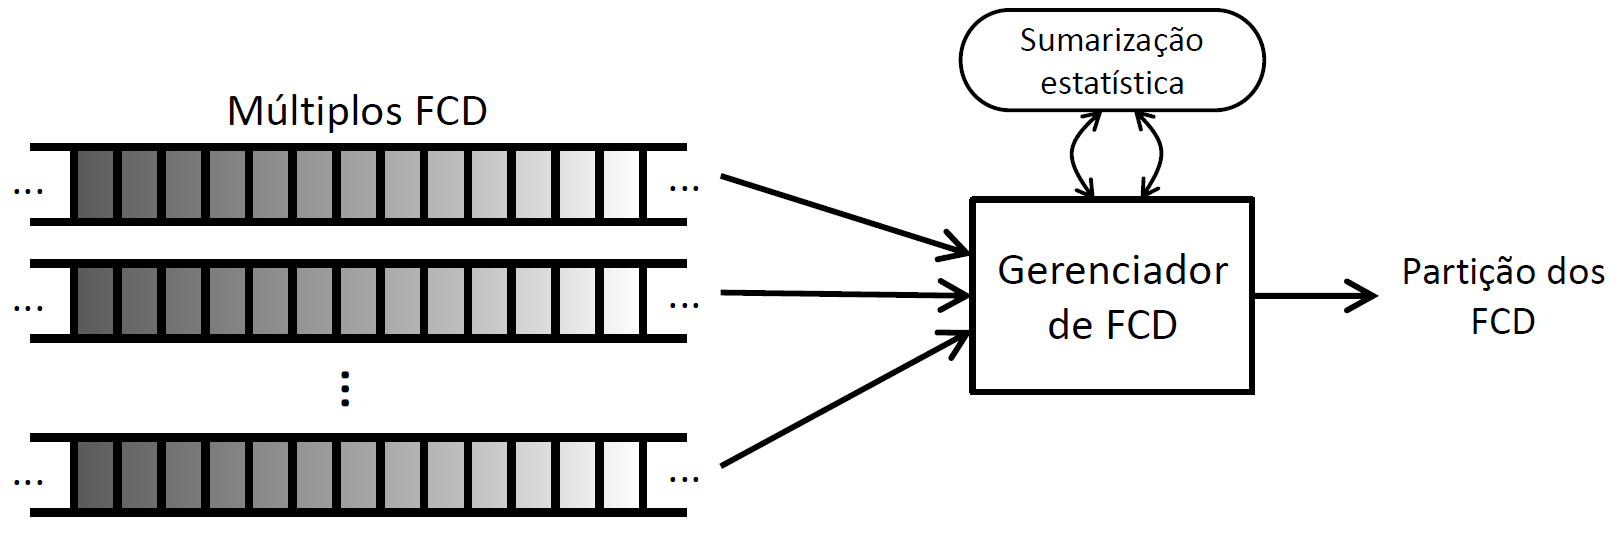
\includegraphics[width=0.7\textwidth]{figures/multiStream}
	\caption{\rewrite{modificar a figura, se for mantida}\emph{Framework} para agrupamento baseado em atributo (múltiplos FD) \cite{Silva2013}}\label{Fig:AgrupMultiStream}
\end{figure}

Estratégias de aprendizado supervisionado de múltiplos FD seguem esquema similar, porém considerando a informação de rótulo de cada fluxo como objetivo do aprendizado. O aprendizado semissupervisionado surge como parte de esforços para a proposta de mecanismos capazes de aprender a partir de múltiplos FDs.

\citeonline{Chen2013} propõem uma estrutura de sumarização para a representação de exemplos de FDs de forma compacta com o objetivo de agrupar múltiplos FDs de forma não supervisionada. O algoritmo \emph{MINETRAC} \cite{Casas2011} combina técnicas de aprendizado não supervisionado e semissupervisionado para identificação e classificação de diferentes classes de fluxos de tráfego de internet, que possuam características similares. Um método semissupervisionado baseado em grafo \cite{Li2014} para propagação de rótulos e extensão do conjunto rotulado que realiza o treinamento de um classificador usando \emph{Support Vector Machine} é utilizado para a identificação de padrões em sequências de dados.

As técnicas que seguem a abordagem de aprendizado baseado em exemplos tem como objetivo criar um modelo correspondente aos dados de um FD único.}

\rewrite{FIM - sobre AFD baseado em atributos vs baseado em exemplos}

\section{Estruturas de Sumarização de Exemplos} \label{chConceitos:FD:Sumario}

Uma solução para contornar a impossibilidade de armazenamento de todos os exemplos é a criação de sumários ou sinopses da informação encontrada nos dados. Uma grande variedade de técnicas tem sido desenvolvidas para o armazenamento de sumários da informação histórica encontrada em FD. \cite{gama2007}.

É possível manter estatísticas simples de FD, que podem ser computadas de forma incremental. Para definir a média de um FD, por exemplo, precisamos manter o número de observações ($i$) e a soma dos valores encontrados até o momento ($\sum x_i$). Assim, com a chegada de um novo exemplo, a média pode ser calculada de forma incremental, como na \autoref{Eq:mediaRecursiva}.

\begin{equation} \label{Eq:mediaRecursiva}
\bar{x}_{i} = \frac{(i-1) \times \bar{x}_{i-1} +  x_{i}}{i}
\end{equation}

De maneira semelhante podem ser definidas outras estatísticas, como desvio padrão e coeficiente de correlação entre dois fluxos. O interessante nessas fórmulas é poder manter estatísticas exatas sobre uma sequência de dados potencialmente infinita sem ter que armazenar todos os dados \cite{gama2007}.

As estruturas de sumarização mais frequentemente utilizadas por técnicas de agrupamento em FD são detalhadas a seguir.

\paragraph{Vetor de Atributos \\}

O uso de vetores de atributos para sumarização de grandes volumes de dados foi introduzido no algoritmo \emph{BIRCH} \cite{zhang1996}. Este vetor, chamado de \emph{Clustering Feature} (CF), conta com três componentes: o número de exemplos ($N$), a soma linear dos exemplos ($LN$) e a soma quadrática dos exemplos ($SS$), sendo que $LS$ e $SS$ são estruturas $n$-dimensionais, de acordo com o número de atributos do FD. Essas componentes permitem o cálculo de métricas de grupo, como média, raio e diâmetro do grupo. 

O vetor CF possui propriedades de incrementais e aditivas, ou seja, é possível inserir um novo exemplo em um CF pela atualização das estatísticas e dois CF podem ser mesclados em um terceiro vetor CF de forma simples.

Algumas abordagens de aprendizado em FD utilizam o vetor CF como descrito nesta descrição, por vezes incluindo pesos para ponderar os grupos \cite{Cao2006,Kranen2011}. Entretanto, há outras abordagens que utilizam variações do CF, a fim de produzir outras estatísticas.

A estrutura nomeada microgrupo, usada primeiramente no algoritmo \emph{CluStream} \cite{Aggarwal2003}, estende o conceito do vetor CF, adicionando mais duas componentes ao CF original: a soma de marcas temporais ou \emph{timestamps} ($LST$) e a soma quadrática de \emph{timestamps} ($SST$). As duas novas componentes tem o objetivo de incluir aspecto temporal na descrição de grupos, que pode ser utilizado para identificar \emph{outliers} ou desvios de conceito.

A proposta do algoritmo \emph{SWClustering} \cite{Zhou2008} também sugere uma extensão para o vetor CF, chamada de \emph{Temporal CF}, que adiciona uma nova componente ao CF original: a \emph{timestamp} do exemplo mais recente a ser inserido no grupo.

Algoritmos que fazem uso de microgrupos ainda podem manter um histórico dessas estruturas para determinar \emph{snapshots} do FD, i.e., recuperar a situação da partição de grupos em um determinado momento no tempo. \cite{aggarwal2007:Ch2}

\paragraph{Arranjos de Protótipos \\}

Alguns algoritmos de agrupamento utilizam uma estrutura simplificada chamada Arranjos de Protótipos, que consiste em um conjunto de protótipos (medóides, centróides, etc) que sumarizam a partição dos dados.

O algoritmo STREAM \cite{Guha2000} divide o FD em partes (\emph{chunks}) e, para cada uma das partes, são definidos $2k$ exemplos representantes obtidos por uma variante do algoritmo $k$-medóides \cite{Kaufman1990}. Esse processo é repetido até que seja completado um conjunto de $m$ exemplos e, então, o agrupamento é aplicado aos protótipos com o objetivo de reduzir esse conjunto.

Estratégia similar é utilizada para o algoritmo \emph{Stream LSearch} \cite{OCallaghan2002}, que os protótipos em memória. Quando a memória está cheia, o conjunto de protótipos é agrupado a fim de manter na memória apenas um subconjunto de protótipos.

\paragraph{Grades de Dados \\}

A sumarização dos exemplos de um FD também pode ser feita por meio de grades \cite{Cao2006,Chen2007,gama2011}, ou seja, pelo particionamento do espaço $n$-dimensional de atributos em células grade de densidade.

Uma estratégia \cite{Chen2007} para a utilização de grades é a associação de um coeficiente de densidade que decresce com o tempo. A densidade de uma célula de grade é determinada pela soma das densidades de cada exemplo inserido na grade. Cada célula é representada por uma tupla $<tg,tm,D,label,status>$, onde $tg$ é a última vez que a célula foi atualizada, $tm$ é a última vez que a célula foi removida do conjunto de células válidas (não \emph{outliers}), $D$ é a densidade desde a última atualização, $label$ é o rótulo de classe da célula e $status$ indica se é uma célula normal ou esporádica (células com poucos objetos, \emph{outliers}).

A manutenção das células de grade é realizada durante a fase \emph{online}. Uma célula pode se tornar esparsa se não receber exemplos por muito tempo e uma célula esparsa pode se tornar densa se receber muitos exemplos. Quando um novo exemplo chega, é verificado a célula a qual pertence e estrutura da célula é atualizada. Células com o $status$ esporádico são removidas periodicamente.

\rewrite{Aspecto não estacionário dos conjuntos: Aprendizado baseado em janelas (mais recente = mais importante, menos recente = menos importante) vs detecção de desvios de conceito}

\section{Desvios de Conceito} \label{chConceitos:FD:Desvios}

Na maioria das aplicações do mundo real, os dados são coletados durante um período de tempo. Para longos períodos, é plausível considerar que os exemplos não são independentes ou não possuem mesma distribuição. Em domínios complexos, é provável que a distribuição de classes mude de acordo com o tempo \cite{Gama2004}. Essas mudanças são conhecidas como desvios de conceito.

Desvios de conceito podem ser graduais, onde há uma transição suave entre as distribuições, ou abruptas, quando a distribuição muda repentinamente.

Abordagens que lidam com desvios de conceitos podem ser classificadas em duas categorias: aquelas que adaptam o modelo em intervalos regulares sem considerar que mudanças ocorreram e aquelas que primeiro detectam desvios de conceitos e, então, adaptam o modelo a essas mudanças. As abordagens da primeira categoria são aquelas que utilizam modelos de janelas temporais.

As estratégias que realizam a detecção de mudanças para posterior adaptação do modelo mantêm um monitoramento, realizado pela definição de indicadores baseados no modelo. Se um desvio é detectado durante o monitoramento, são aplicadas ações para a adaptação do modelo de aprendizado.

Os trabalhos \cite{Gama2004,Li2012,wu2012} trazem maiores informações sobre algumas estratégias de detecção de desvios de conceito.

\subsection*{Janelas Temporais} \label{chConceitos:FD:Janelas}

As janelas temporais são uma abordagem bastante utilizada para resolver a questão de conjuntos abertos (infinitos) como FD. Ao invés do considerar todo o conjunto de exemplos de um fluxo, são considerados subconjuntos de exemplos ao longo do tempo. Neste modelo, uma marca temporal está associada a cada exemplo, a fim de determinar se o exemplo é válido ou não, ou seja, se está dentro ou fora de uma determinada janela temporal.

Existem diferentes modelos de janelas que podem ser encontrados na literatura, os mais relevantes \cite{Zhu2002} são descritos a seguir:

\begin{description}
\item[Modelo \emph{Sliding Window}:] neste modelo apenas a informação mais recente do FD é armazenada em uma estrutura de dados (janela) cujo tamanho pode ser variável ou fixo. Esta é uma estrutura tipo \emph{First In, First Out}, que considera os exemplos de um determinado ponto no tempo atual até um ponto no passado. A \autoref{Fig:slidingWindow} traz um exemplo do modelo \emph{Sliding Window}, com comprimento fixo de janela, em três momentos do tempo ($t-2$, $t-1$ e $t$) representando o deslizamento da janela para que contenha os exemplos mais recentes no tempo mais atual $t$. Algoritmos que utilizam este modelo \cite{Ren2009} apenas atualizam os sumários estatísticos dos exemplos dentro da janela.

\item[Modelo \emph{Damped Window}:] também conhecido como \emph{time-fading}, este modelo considera a informação mais recente pela associação de pesos aos exemplos do FD \cite{Jiang2006}: exemplos mais recentes tem peso maior que exemplos mais antigos e o peso dos exemplos diminui de acordo com o tempo. Um exemplo pode ser visualizado na \autoref{Fig:dampedWindow}, que mostra o decaimento do peso de acordo com o degradê dos exemplos. Algoritmos \cite{Cao2006,Chen2007,Isaksson2012} baseados nesse modelo usualmente adotam uma função exponencial de decaimento para o peso dos exemplos.

\item[Modelo \emph{Landmark Window}:] o processamento, neste modelo, se faz por porções disjuntas do FD, nomeadas \emph{chunks}, que são separadas de acordo com a ocorrência de \emph{landmarks} (aparecimento de exemplos relevantes). Os \emph{landmarks} podem ser definidos de acordo com o tempo, e.g., diário ou semanal, ou quanto ao número de elementos observados desde o \emph{landmark} anterior. Quando um novo \emph{landmark} é alcançado, todos os exemplos da janela são removidos e novos são adicionados a partir desse momento. Na \autoref{Fig:landmarkWindow} há um exemplo para o modelo. Estratégias possíveis usando este modelo são baseadas na utilização dos modelos obtidos pelos diversos \emph{chunks} em conjunto ou como guias para próximos modelos.
\end{description}

\begin{figure}[!htb]
        \centering
        \begin{subfigure}[t]{0.4\textwidth}
                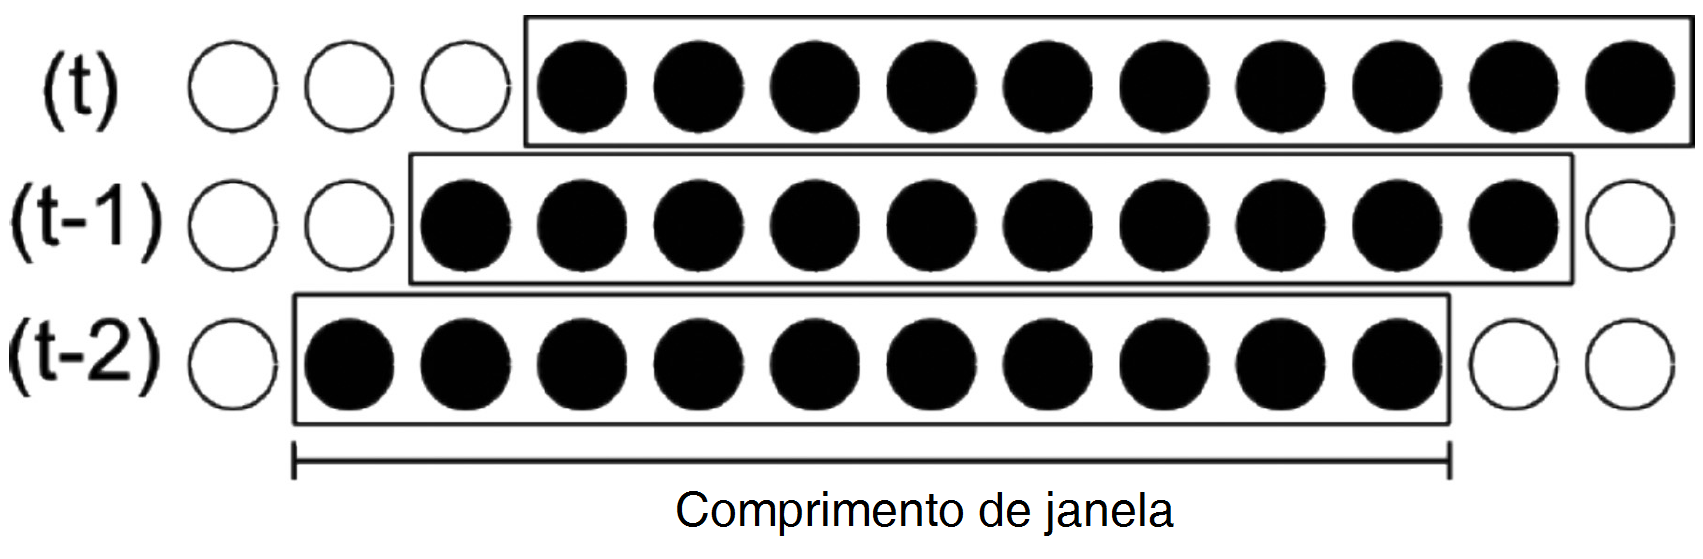
\includegraphics[width=\textwidth]{figures/slidingWindow}
                \caption{Modelo \emph{Sliding Window}}
                \label{Fig:slidingWindow}
        \end{subfigure}%
        \qquad %add desired spacing between images, e. g. ~, \quad, \qquad, \hfill etc.
          %(or a blank line to force the subfigure onto a new line)
        \begin{subfigure}[t]{0.4\textwidth}
                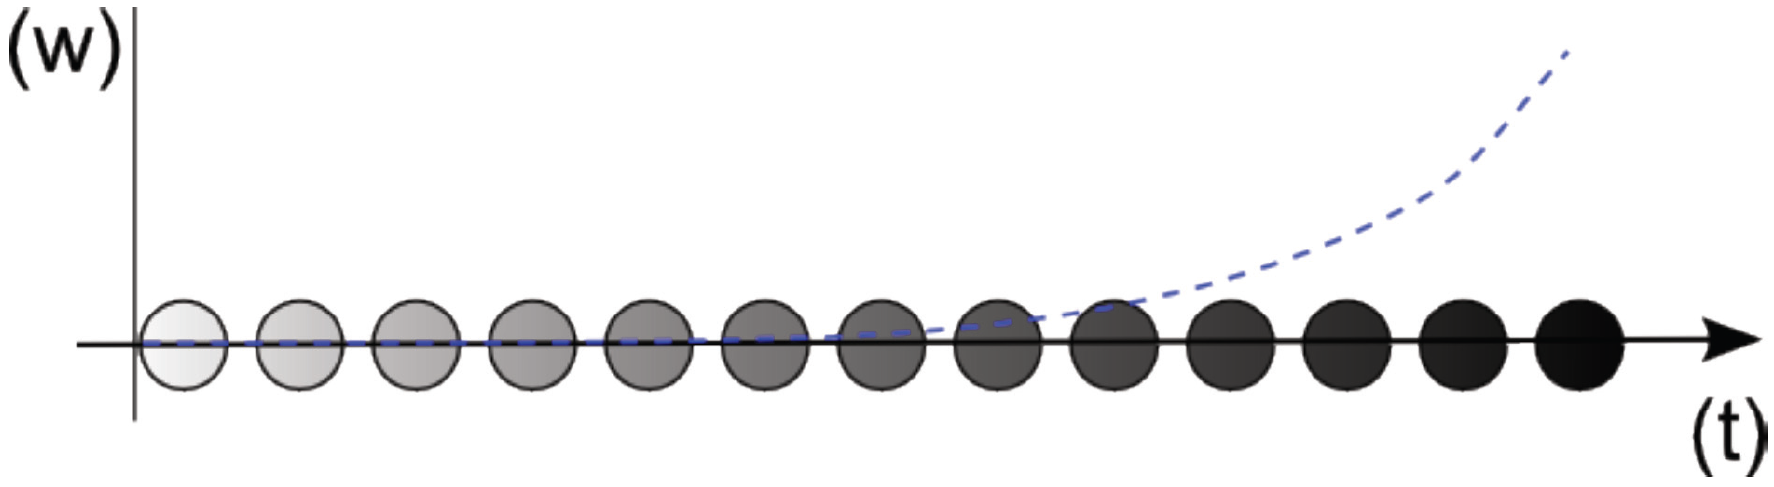
\includegraphics[width=\textwidth]{figures/dampedWindow}
                \caption{Modelo \emph{Damped Window}}
                \label{Fig:dampedWindow}
        \end{subfigure}
        \qquad %add desired spacing between images, e. g. ~, \quad, \qquad, \hfill etc.
        %(or a blank line to force the subfigure onto a new line)
        \begin{subfigure}[t]{0.4\textwidth}
        		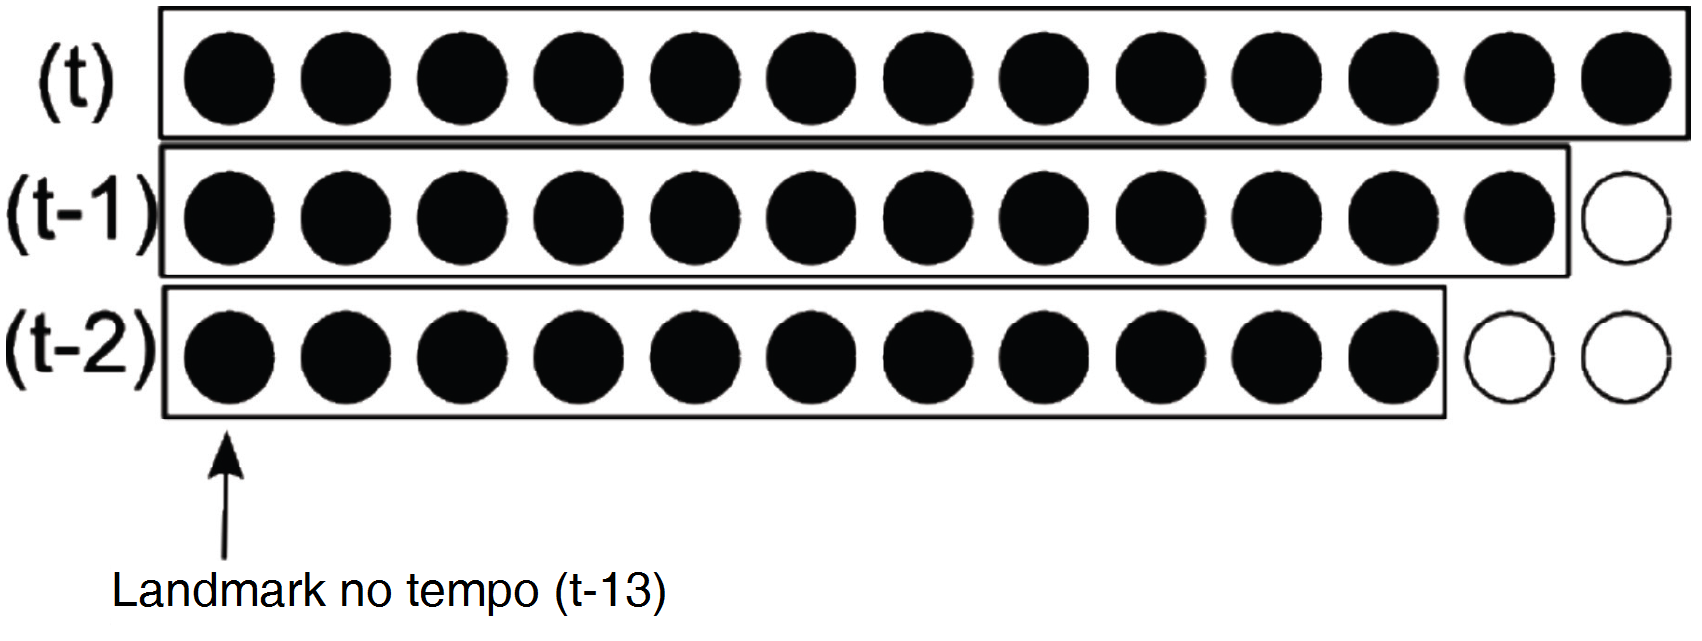
\includegraphics[width=\textwidth]{figures/landmarkWindow}
        		\caption{Modelo \emph{Landmark Window}}
        		\label{Fig:landmarkWindow}
        \end{subfigure}
        \caption{Exemplos ilustrativos de modelos de janela temporal \cite{Silva2013}}\label{Fig:modeloJanelas}
\end{figure}

Além das características mencionadas a respeito do volume de exemplos, há também um componente temporal inerente a aprendizado em FD. Os dados podem evoluir de acordo com o tempo e assim a distribuição do conjunto pode ser alterada. Deste modo, algoritmos que apenas sugerem adaptações para contornar as questões de volume de exemplos podem não ser soluções efetivas neste contexto. Algoritmos de aprendizado em FD devem ter foco claro na evolução dos dados \cite{aggarwal2007:Ch1}.

O uso de modelos de janela temporal podem auxiliar no tratamento de um dos aspectos da evolução dos exemplos do FD, por permitir uma avaliação de acordo com o tempo. No entanto, existem outros aspectos que podem ser explorados. A próxima seção fala sobre a difícil tarefa de identificação de desvios de conceito.

\section{Técnicas de Agrupamento em Fluxos de Dados}

\rewrite{apresentar de outra forma (tabela?), destacar mais relevantes/importantes?}

Abordagens de agrupamento de dados são tipicamente utilizadas no aprendizado não supervisionado. Dentro da área de FD é comum verificar a falta de informação de classe, seja por conta da natureza do domínio (não existem classes definidas) ou pela dificuldade em rotular exemplos de um FD.

Independentemente dos métodos adotados, é desejável que algoritmos de agrupamento em FDs possuam a capacidade de \cite{Amini2014}: 
\begin{enumerate*}[label=\itshape\alph*\upshape)]
\item descobrir grupos de formatos arbitrários;
\item lidar com ruído;
\item realizar o agrupamento sem informação prévia sobre o número de grupos
\end{enumerate*}.

%Há diferentes técnicas para agrupamento em FD e elas podem ser divididas de acordo com a abordagem de agrupamento que seguem.

\rewrite{falar sobre propostas baseada em chunks de exemplos}

\subsection{\emph{Framework Online-Offline} (FOO) para Agrupamento em FD} \label{ChAFD:framework}

Algoritmos de agrupamento baseados em exemplos podem ser resumidos em dois passos \cite{Cao2006,Yang2006}: abstração dos dados (componente\emph{online}) e agrupamento (componente \emph{offline}), ilustrados na \autoref{Fig:onlineOffline}.

\begin{figure}[!htb]
	\centering
	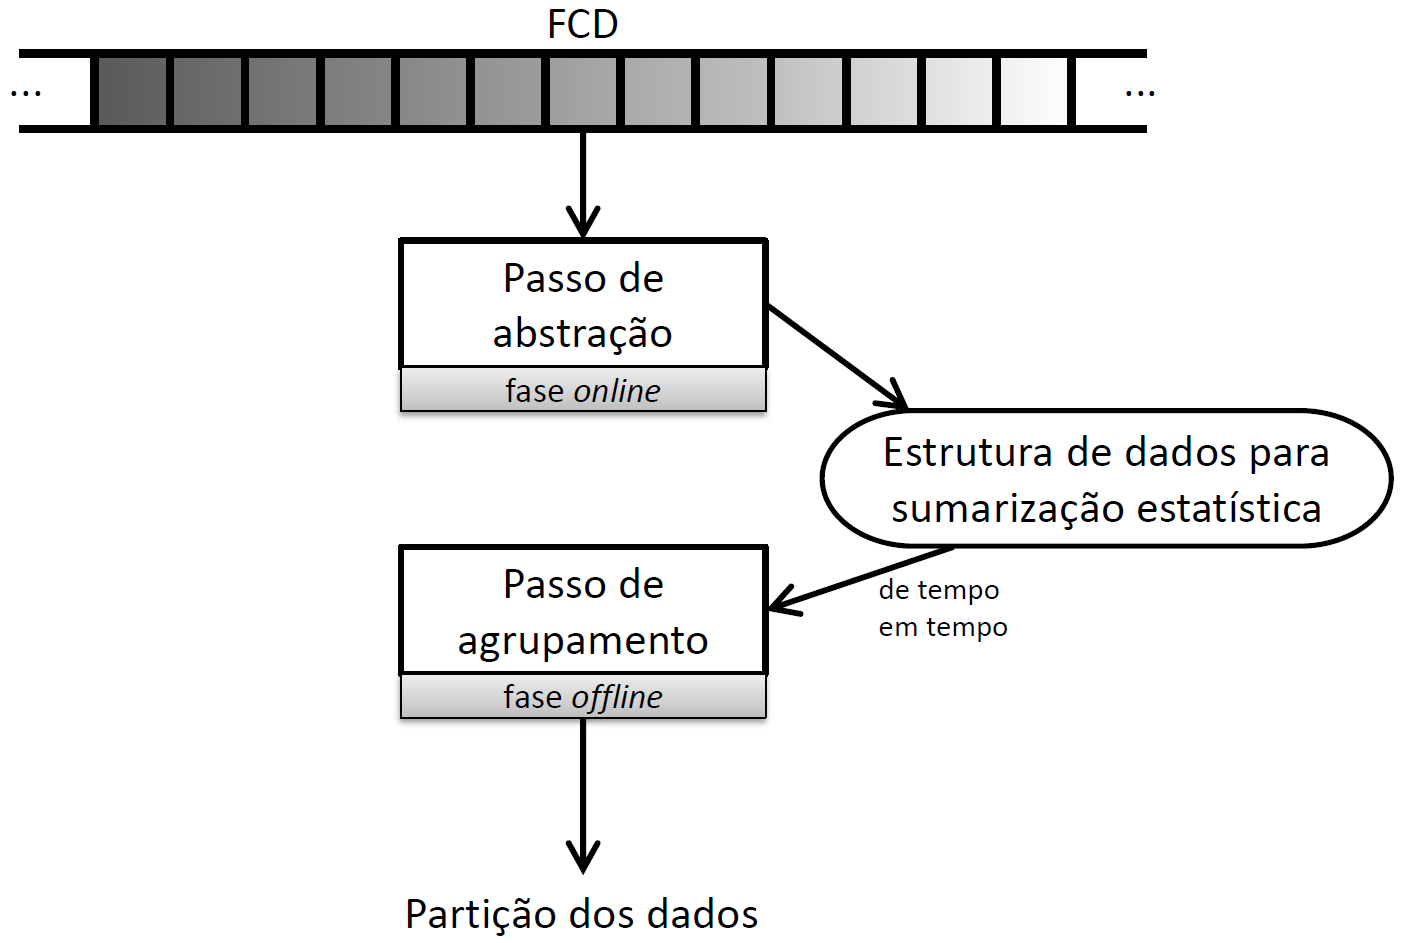
\includegraphics[width=0.7\textwidth]{figures/onlineOffline}
	\caption{\emph{Framework} \emph{online-offline} \cite{Silva2013}}\label{Fig:onlineOffline}
\end{figure}

A fase \emph{online}, abstração dos dados, sumariza os dados do FD com o auxílio de estruturas particulares para lidar com restrições de espaço e memória das aplicações FD. Essas estruturas de sumarizam os dados para preservar o significado dos objetos originais sem a necessidade de armazená-los. Estruturas frequentemente utilizadas são vetores de atributos, arranjos de protótipos e grades de dados. Essas estruturas são melhor detalhadas na \autoref{chConceitos:FD:Sumario}.

Para a contínua sumarização dos exemplos que chegam e dar maior importância aos exemplos mais recentes, uma abordagem popular é a definição de janelas temporais, como apresentado na \autoref{chConceitos:FD:Janelas}.

Durante o passo de abstração, algoritmos de agrupamento em FD devem utilizar mecanismos para detecção de \emph{outliers} que sejam capazes de diferenciar verdadeiros \emph{outliers} de evolução de grupos (\autoref{chConceitos:FD:Desvios}), uma vez que a distribuição dos dados pode variar de acordo com o tempo.

Na fase \emph{offline} é possível obter uma partição dos dados pelo passo de agrupamento. Neste momento, pode ser necessária a definição de alguns valores de entrada (número de grupos, por exemplo) para que seja possível ter uma visão geral dos grupos do FD. Algoritmos de agrupamento tradicionais podem ser utilizados considerando o conjunto de estruturas de sumarização para encontrar uma partição dos dados. O formato dos grupos encontrados está ligado ao algoritmo de agrupamento empregado, por exemplo, o $k$-\emph{means} \cite{macqueen1967} gera grupos hiperesféricos enquanto o DBSCAN \cite{Ester1996} é capaz de descobrir grupos de formatos aleatórios.

O \emph{framework} apresentado nesta seção é frequentemente utilizado para o desenvolvimento de novas técnicas de agrupamento em FD. Algumas dessas propostas são discutidas no \autoref{ChSemi}.

O \emph{ClusTree} \cite{Kranen2011}, por exemplo, é a proposta de uma estrutura hierárquica compacta e auto-adaptativa para manter sumários de FD, construindo uma hierarquia de microgrupos em diferentes níveis. Outras técnicas que seguem a abordagem hierárquica de agrupamento são o \emph{E-Stream} \cite{Udommanetanakit2007}, que possui suporte para cinco tipos de evolução em grupos (aparecimento, desaparecimento, evolução própria, mescla e divisão), e suas extensões para suporte de incerteza (valores faltantes) em FDs heterogêneos (conjuntos que combinam atributos numérico-contínuos e categóricos) \cite{Meesuksabai2011} e FDs de alta dimensão \cite{Chairukwattana2014}.

As subseções a seguir apresentam técnicas já existentes baseadas em agrupamento particional e baseado em densidade, onde é possível identificar focos de pesquisas mais recentes.

\subsection{Agrupamento Particional em FD}

Os algoritmos de agrupamento particional para FD, em sua maioria, são propostos como extensões de algoritmos de agrupamento particionais conhecidos, como $k$-\emph{means}, $k$-medóides e \emph{Affinity Propagation}.

O algoritmo \emph{CluStream} \cite{Aggarwal2003} é baseado no algoritmo $k$-\emph{means} e introduz um \emph{framework} \emph{online-offline} para agrupamento em FD que vem sendo adotado para grande parte dos algoritmos propostos recentemente. \citeonline{Yang2006} propõem uma extensão chamada \emph{HCluStream} para lidar com FDs heterogêneos.

A proposta de \citeonline{Labroche2014} está baseada no algoritmo $k$-medóides e realiza agrupamento \emph{fuzzy} de forma incremental. O trabalho de \citeonline{Lemos2013} apresenta uma técnica para geração de um classificador \emph{fuzzy} baseado em agrupamento incremental para a geração de regras que descrevem novos estados operacionais de um sistema de detecção e diagnóstico de falhas.

\citeonline{Hore2007} apresentam a proposta de uma abordagem genérica para agrupamento iterativo \emph{fuzzy}/possibilístico em FD, introduzindo equações objetivo transformadas para os algoritmo FCM \cite{Bezdek1981}, \emph{possibilitistc $c$-means} \cite{Krishnapuram1996} e Gustafson-Kessel \cite{Gustafson1978}. Outro trabalho \cite{Hore2007a} traz uma nova variante do FCM para aprendizado em FD, o \emph{Streaming} FCM, que realiza adaptação à evolução de distribuições pela utilização de uma parte do histórico de protótipos/centróides no agrupamento de \emph{chunks} de dados, conforme sua chegada. Em \cite{Hore2008} é explorada uma extensão \emph{online} para o FCM que mantém sumarização do agrupamento usando exemplos ponderados. Os exemplos ponderados obtidos pelo agrupamento de cada \emph{chunk} de dados formam um \emph{ensemble} que é transformado em um conjunto de grupos finais.

Alguns trabalhos propõem algoritmos baseados no agrupamento \emph{Affinity Propagation} (AP) \cite{Frey2007}. Usando método de passagem de mensagem, o AP escolhe, entre os exemplos disponíveis, aqueles que melhor representam o conjunto, os chamados \emph{exemplars}, que indicam os diferentes grupos dentro do conjunto de exemplos. Com os \emph{exemplars} não é necessário definir o número de grupos inicialmente.

Uma extensão do AP  para aprendizado em FD é o algoritmo \emph{Streaming} AP \cite{Zhang2008}. Esta proposta é dividida em dois passos, sendo que o objetivo do primeiro é encontrar os \emph{exemplars} ponderados dentro de um \emph{chunk} de dados por uma extensão do AP (\emph{Weighted Affinity Propagation}), enquanto o segundo visa diminuir a complexidade do modelo pela aplicação do \emph{Weighted Affinity Propagation} para o conjunto de \emph{exemplars}. Em trabalho mais recente \cite{Zhang2014}, o \emph{Streaming} AP traz melhorias como mecanismo de detecção de mudanças e adaptação do modelo da distribução dos dados.  

\subsection{Agrupamento Baseado em Densidade em FD}

Os algoritmos baseados em densidade também são utilizados como alternativa para a tarefa de agrupamento, sendo duas de suas vantagens a alta tolerância a ruído ou \emph{outliers} e a habilidade em descobrir grupos de formatos arbitrários.

As técnicas de agrupamento baseado em densidade seguem, comumente, duas abordagens que são descritas nas próximas seções e incluem exemplos de algoritmos que se encaixam nessas categorias.

\subsection{Algoritmos de Microgrupos de Densidade}

Em algoritmos de agrupamento de microgrupos de densidade, microgrupos mantêm a informação de sumarização dos exemplos e o agrupamento é realizado usando as estruturas de sinopse.

A proposta de \citeonline{Cao2006} é o algoritmo de agrupamento em FD baseado em densidade chamado \emph{DenStream}, que utiliza duas estruturas de sumarização para lidar com novas distribuições no FD, diferenciando-as de \emph{outliers}. As estruturas nomeadas \emph{core-micro-cluster} (cmc), referentes ao agrupamento em si, e \emph{pontential core-micro-cluster} (pcmc), distribuição de exemplos que representa regiões menos densas que são mantidas. O aprendizado da estrutura do FD é realizado em duas fases. Na fase \emph{online} do algoritmo, cada novo exemplo pode ser associado a um microgrupo já existente (cmc ou pcmc), de acordo com cálculo de métrica de dissimilaridade (distância Euclidiana) ou será criado um novo pcmc para o novo exemplo. Na fase \emph{offline} é aplicado o algoritmo \emph{DBSCAN} \cite{Ester1996} para determinar o grupos finais, de acordo com o conjunto de cmc. De tempos em tempos, um método de poda avalia o conjunto de pcmc para garantir que são \emph{outliers}, de acordo com a densidade, e descartá-los. O \emph{DenStream} não possui mecanismos para a eliminação de microgrupos ou para fundir dois ou mais microgrupos, o que pode ser problemático conforme o crescimento do conjunto de exemplos e limitações de espaço para armazenamento.

O \emph{DenStream} serviu de inspiração para outras técnicas que consideram situações particulares e implementam adaptações para lidar com contextos diversos. \citeonline{LiXiong2009} desenvolveram um algoritmo baseado no \emph{DenStream} para aplicações com grande volume de outliers. %O \emph{rDenStream} gera um classificador com base no resultado do agrupamento. Em um passo específico do algoritmo, dados inicialmente descartados têm a chance de ser reaprendidos. Nesta técnica os pcmc não são descartados, formando um conjunto de histórico de \emph{outliers}, o que resulta na necessidade de mais espaço para manter o histórico.
O algoritmo \emph{SDStream} \cite{Ren2009}  tem a habilidade de descobrir grupos de formatos arbitrários dentro de um modelo de janela deslizante, que permite o esquecimento progressivo dos dados antigos. %Durante o processo de aprendizagem, a distribuição dos dados mais recentes do FD é considerada e os exemplos que não mais pertencem à janela de tempo considerada são descartados. A utilização do modelo de janela deslizante permite o esquecimento dos dados antigos, pois assume-se que o interesse do usuário está na distribuição dos dados mais recentes do FD.
\emph{HDenStream} \cite{Lin2009} é um algoritmo adaptado para aprendizado em FDs com atributos heterogêneos pela inclusão de um atributo bidimensional para manter a frequência de atributos categóricos. %A técnica oferece possível solução para aplicações onde existem dados categóricos e contínuos.
O \emph{HDDStream} \cite{Ntoutsi2012} traz adaptações ao original \emph{DenStream} para melhorar o agrupamento de FDs de alta dimensão. O \emph{PreDeConStream} \cite{Hassani2012} melhora a eficiência da fase \emph{offline} do \emph{HDDStream}.

Alguns métodos híbridos utilizam conceitos do algoritmo \emph{DenStream} aliado a outras abordagens. O \emph{StreamOptics} \cite{Tasoulis2007} é um \emph{framework} baseado nos conceitos de cmc e pcmc, que utiliza o algoritmo \emph{OPTICS} \cite{Ankerst1999} para produzir visualização gráfica da estrutura do FD e sua evolução com o passar do tempo. No entanto, em nenhum momento é gerada uma partição do conjunto, então a análise do agrupamento deve ser realizada manualmente. \citeonline{Isaksson2012} propõem o algoritmo \emph{SOStream}, que detecta estrutura de FDs de rápida evolução pela adaptação automática de limiar para o agrupamento baseado em densidade. O limiar é individual por grupo e é definido automaticamente dentro do processo de agrupamento, baseado na ideia de construir vizinhanças com um mínimo de pontos, como parte da análise para criação, remoção,mescla e divisão de grupos. O algoritmo utiliza aprendizado competitivo como em \emph{Self Organizing Maps} \cite{Kohonen1982}, o que pode tornar o processo mais oneroso.

O algoritmo \emph{APDenStream} \cite{Zhang2013} baseia-se nos métodos AP e \emph{DenStream} para definição de um modelo geral que representa o FD. O algoritmo AP substitui o \emph{DBSCAN} na fase \emph{offline} do \emph{DenStream}. Baseado em trabalho anterior dos autores \cite{Forestiero2009}, FlockStream \cite{Forestiero2013} utiliza um sistema multi-agente baseado em um modelo de \emph{flocking} \cite{Kennedy2001}. Nesta técnica os agentes são microgrupos que trabalham de forma independente mas formam grupos juntos.

\subsection{Algoritmos Baseados em Densidade e Grades}

Em se tratando de agrupamento não supervisionado de FDs é possível identificar recente tendência no investimento de abordagens baseadas em grades e densidade \cite{Amini2011,Amini2014}.

%Grande parte das técnicas de agrupamento baseadas em grade e densidade seguem o fOO, mapeando os exemplos em células do espaço de atributos (grades) que são agrupadas de acordo com suas densidades. 
Uma das primeiras tentativas de associar os dois métodos foi o trabalho de \citeonline{Gao2005}, que propõe um algoritmo de agrupamento incremental de passagem única usando células do espaço de atributos (grades) densas que são consideradas em uma fase de agrupamento caso tenham valor de densidade acima de um limiar pré-definido.

O \emph{D-Stream} \cite{Chen2007, Tu2009} é uma proposta de agurpamento em tempo real baseado em grades, apoiado no fOO. Na fase \emph{online} acontece a leitura de um novo exemplo e seu mapeamento na grade. Na fase \emph{offline} os grupos são criados e ajustados em intervalos. No primeiro ciclo cada grade considerada densa é associada a um grupo distinto, nos intervalos seguintes os grupos são ajustados. O ajuste de grupos acontece por meio da identificação de grades densas e esparsas: grades densas são mescladas a grades vizinhas, formando um grupo; caso contrário a grade é removida do grupo. O método, que agrupa os exemplos em tempo real, inclui mecanismos para decaimento de densidade com a passagem do tempo, detecção de evolução de comportamento e tratamento de \emph{outliers}.

\rewrite{é aqui que eu comento do problema das grades? Tamanho da grade (como dividir o espaço), número de dimensões/atributos (grades esparsas > grades densas, mais oneroso para manter em memória e fase offline (volume de grade e verificação de grupos)}

\rewrite{O D-Stream é o principal baseado em grade e densidade, os outros podem aparecer somente na tabela, se for o caso de mencionar}

%Algumas extensões para o \emph{D-Stream I} são propostas. \citeonline{Jia2008} propuseram um modelo que melhora a qualidade dos grupos pela detecção dos pontos limites de uma grade. A extensão \emph{D-Stream II} \cite{Tu2009} inclui uma restrição de atração entre grades para a mesclagem e composição de um grupo na fase \emph{offline}. A atração entre grades é verificada pela construção de hipercubos centrados nos exemplos de uma grade, considerando cada atributo do FD, a fim de estabelecer um volume para a grade, que será utilizada para verificar se duas grades devem ou não ser mescladas em um mesmo grupo.

%Ao realizar agrupamento baseado em grades, quanto maior a dimensão do conjunto de dados, maior o número de grades vazias. Pensando nisso, \citeonline{Ren2011} propõem o algoritmo \emph{PKS-Stream} para conjuntos de alta dimensão. A técnica possui uma estrutura de árvore para manter as grades não-vazias e suas relações. À chegada de um novo exemplo, o algoritmo verifica as estruturas de sumarização de grade para ver se o exemplo pertence a alguma das grades existentes na estrutura de árvore. Caso não seja verdadeiro, um novo elemento de sumarização de grade é criado. De tempo em tempo, a árvore é ajustada, pela remoção de grades esparsas, e os grupos são formados de acordo com a densidade das grades vizinhas. O \emph{PKS-Stream I} \cite{Zhang2012a} é uma versão otimizada do \emph{PKS-Stream} quanto à seleção de período para detecção de densidade, identificação e remoção esporádica de grades.

%\emph{DCUStream} \cite{Yang2012} é um algoritmo baseado em densidade e grades para aprendizado em FDs com dados incertos. A proposta introduz o conceito de \emph{core dense grid} que é uma grade densa com vizinhos esparsos, usados no momento de agrupamento na fase \emph{offline}, quando os vizinhos esparsos são considerados ruído. O processo de busca pelos \emph{core dense grids} e seus vizinhos pode ser bastante lento.

%A proposta do algoritmo \emph{DENGRIS-Stream} \cite{Amini2012} realiza o agrupamento dentro de um modelo de janela deslizante, na tentativa de capturar a distribuição mais recente dos dados. É a primeira proposta para agrupamento baseado em densidade e grades que considera o modelo de janela deslizante.

%\emph{ExCC} \cite{Bhatnagar2013} é um algoritmo de agrupamento baseado em densidade e grades que tem como foco o aprendizado em FDs heterogêneos. O algoritmo é robusto, adaptando-se a mudanças na distribuição dos dados e detectando \emph{outliers} com rapidez. O algoritmo implementa um mecanismo para garantir o curso de novos grupos descobertos.

Pela revisão aqui exposta, pode-se verificar que é crescente o número de novas propostas para agrupamento em FDs, em especial aquelas que utilizam abordagem baseada em densidade e outras abordagens capazes de lidar com o surgimento e desaparecimento de grupos de forma simples.

No entanto, neste tipo de aprendizado, é ignorada qualquer informação prévia que possa existir a respeito da distribuição dos dados. O investimento em novas propostas para aprendizado semissupervisionado em FD também cresceu nos últimos anos, como pode ser inferido pelas técnicas apresentadas na próxima seção.

\section{Agrupamento Fuzzy em Fluxo de Dados}

O método não supervisionado de agrupamento \emph{Single Pass Fuzzy C Means} (SPFCM) \cite{Hore2007b} tem como objetivo oferecer uma alternativa ao agrupamento FCM para conjuntos de dados cujo grande tamanho impede seu armazenamento total em memória para a aplicação do processo de agrupamento. A técnica parte do princípio de que os dados do conjunto estão disponíveis em partes, nomeadas \emph{chunks}, às quais são processadas pelo algoritmo WFCM. 

O \autoref{algo:SPFCM} apresenta os passos gerais para a proposta. Quando chega o primeiro \emph{chunk} todos os exemplos possuem peso de valor 1 (um). Após a aplicação do WFCM calcula-se o peso para cada centróide obtido, com base na matriz de pertinência. Os centróides serão adicionados ao próximo \emph{chunk} de novos exemplos e o agrupamento WFCM é aplicado ao conjunto resultante dessa união.

\begin{algorithm2e}[!htb]
	\SetAlgoLined
	\Entrada{$E$, $k$, $m$, $n_{s}$}
	\Saida{$U$, $C$}
	\Inicio{
		$U = $ geraMatrizPertinênciaAleatória()\;
		$C = $ geraCentróidesIniciais($E$, $U$)\;
		$E' = $ gerarSubconjuntosExemplos($E$, $n$)\;
		$w = 1_{n_{s}}$\;
		$U, C = $ WFCM($E'[1]$,$k$,$m$,$w$)\;
		PAREI AQUI \;
		\Enqto{$\epsilon > \xi$}{
			atualizarMatrizPertinência($U$)\;
			$C'= C$\;
			atualizarCentróides($C$)\;
			$\epsilon = max_{1 \leq i \leq k}\{\| c_{i} - c'_{i} \|^{2}\}$\;
		}
	}
	\caption{\emph{Single-Pass Fuzzy} $C$-\emph{Means} (SPFCM) \cite{Hore2007b}} \label{algo:SPFCM}
\end{algorithm2e}

%O vetor $w$ é um conjunto pesos $\{w_{1}, w_{2}, ..., w_{n}\}$, onde $w_{j} \geq 0$ determina a influência de cada exemplo $e_{j}$ para o processo de agrupamento.

%As atualizações para a matriz de pertinência seguem a Equação \ref{eq:fcmAtualizaU} e geração inicial e atualização dos centróides é calculada pela Equação \ref{eq:spfcmAtualizaW} e a

%\begin{equation}
%	c_{i} = \frac{\sum_{j=1}^{n} w_{j}u_{ij}^{m}e_{j}}{\sum_{j=1}^{n} w_{j}u_{ij}^{m}}
%	\label{eq:spfcmAtualizaW}
%\end{equation}

O SPFCM contempla a dificuldade de armazenamento de exemplos, processando \emph{chunks} do conjunto e eliminando os exemplos logo após a obtenção dos centróides ponderados. No entanto, é uma técnica que considera que a distribuição dos dados é estática, o que deixa de lado a característica mutável do contexto de FD.

Os autores do SPFCM propõem, então, uma variação do algoritmo\cite{Hore2007} que inclui um mecanismo para lidar com o aspecto não estacionário dos FD. Nesta nova técnica, a partir do segundo \emph{chunk} de dados, os pesos dos centróides são calculados a partir da matriz de pertinência para os exemplos novos apenas, desconsiderando os centróides ponderados, que servem apenas como histórico de agrupamentos anteriores.

A técnica variante do SPFCM é capaz de lidar com quantidades diferentes de histórico, incorporando ao \emph{chunk} de novos exemplos $h$ conjuntos de centróides ponderados obtidos anteriormente. Uma das dificuldades nessa estratégia é determinar o valor de $h$, uma vez que essa definição depende do domínio ao qual é aplicado o agrupamento.

Outra complicação de estratégias baseadas no SPFCM é a definição prévia de um número fixo de grupos, pois, uma vez que um FD é mutável de acordo com o tempo pode ocorrer o aumento ou diminuição no número de grupos. Outro obstáculo: identificação de grupos de formato arbitrário (?)

\rewrite{
número fixo de grupos

sumarização por protótipos - centróides ponderandos (ponderação baseada na matriz de pertinência)

histórico - união de $h$ conjuntos de centróides ao novo \emph{chunk de exemplos}
}

\rewrite{

\section{Considerações Finais}

}
\chapter{Semissupervisão no Aprendizado em Fluxo de Dados} \label{ChSemi}

%Tendo em conta os aspectos envolvidos no aprendizado em FD e o recente crescimento de esforços para encontrar soluções capazes de lidar com os desafios encontrados nesta variedade de domínios, evidenciado na \autoref{chConceitos:FD}, julga-se interessante a investigação mais aprofundada das diversas propostas existentes na literatura para aprendizado em FD.

%As propostas de técnicas para aprendizado em FD são, na maioria das vezes, adaptações de técnicas de aprendizado clássico para lidar com um ou mais desafios encontrados em domínios de FD, e.g.: a necessidade de processar os dados logo que chegam, seja de forma \emph{online} (exemplo a exemplo) ou considerando partes do conjunto de exemplos (processamento de \emph{chunks}); a adaptação do modelo geral que representa o FD e a otimização de suas estruturas; a detecção e tratamento de desvios de conceito.

%Algumas técnicas de aprendizado incremental foram desenvolvidas para domínios específicos ou com foco em conjuntos de dados que, embora volumosos, não apresentam características de FD, como, por exemplo, questões de desvio de conceito. Ainda que o foco principal das propostas não seja o aprendizado em FD, certas abordagens podem ser aplicadas neste contexto, porém com algumas ressalvas, já que não possuem mecanismos para lidar com um ou outro aspecto intrínseco aos domínios FD.

%Este capítulo apresenta discussão sobre uma revisão bibliográfica de abordagens para aprendizado em FD organizadas de acordo com as suas principais características, desenvolvidas especificamente com este intuito ou não. As técnicas colocadas neste capítulo consideram a abordagem de aprendizado por exemplos, em que o processo de aprendizagem tem seu foco nas instâncias de um único FD.

%\section{Técnicas de Classificação em Fluxos de Dados}

%No caso em que o FD envolve dados rotulados, o aprendizado pode ser feito por meio de técnicas supervisionadas. Encontra-se na literatura um volume significativo de trabalhos que utilizam a indução de modelos baseados em árvores. Outros trabalhos abordam o assunto propondo a criação de modelos híbridos utilizando conceitos \emph{fuzzy}. Outra abordagem bastante explorada nesse contexto é a integração de múltiplos modelos. A seguir, alguns trabalhos representativos dessa categoria são apresentados.
%%\undecided{\subsection{Aprendizado Supervisionado em FD baseado em Árvores}}
%
%A indução de árvores de decisão é uma forma de aprendizado supervisionado amplamente utilizada e tem sido bastante explorada dentro do contexto de FDs. Muitas das propostas envolvendo árvores de decisão utilizam ideias gerais das AH, apresentadas na \autoref{chConceitos:FD:HoeffdingTrees}.
%
%O algoritmo \emph{Incremental Extremely Random Forest} \cite{Wang2009} considera o aprendizado, feito por árvore de decisão baseada em AH, em FDs com baixo volume de exemplos, mas em domínios onde seja necessária a adaptação do modelo geral de classificação.
%
%A \emph{Very Fast Decision Tree} (VFDT) \cite{Domingos2000}, uma proposta de aprendizado incremental baseada em AH, serviu de fundamento para outros métodos.  A abordagem utiliza limiares de Hoeffding para garantir que a saída de suas árvores seja o mais próxima de um classificador convencional, que aprende a partir de conjuntos estáticos.
%
%Uma das propostas que utiliza VFDT é a \emph{Concept-adapting Very Fast Decision Tree} (CVFDT) \cite{Hulten2001}, que tem como foco a detecção e adaptação a desvios de conceito em FDs. \citeonline{Liu2009} apresentam uma proposta de um mecanismo para integração de ambiguidades à CVFDT, modificando a divisão de nós pela exploração de múltiplas opções. A técnica visa garantir que o conhecimento mais novo seja utilizado na divisão dos nós, mas também é capaz de reaprender conceitos ressurgentes.
%
%\citeonline{Tsai2009} apresentam uma proposta diferenciada para mineração de regras de desvios de conceitos, buscando encontrar a regra que governa o desvio identificado. A mineração de regras de conceito é feita pelo algoritmo CDR-Tree, que considera dois blocos de dados de um FD que dizem respeito aos mesmos indivíduos em tempos distintos. A partir dos exemplos de cada bloco, o algoritmo forma pares que serão utilizados para a construção de uma árvore de decisão tradicional. As regras de desvio de conceito são mineradas a partir da árvore construída com os pares de exemplos velhos (bloco de dados no tempo $\delta$) e novos (bloco de dados no tempo $\delta + t$). No mesmo trabalho são propostas estratégias para diminuir a complexidade das regras de desvio de conceito mineradas.
%
%%\undecided{\subsection{Aprendizado Supervisionado em FD que utilizam Fuzzy}}
%
%Dentro do conjunto de abordagens para aprendizado supervisionado em FD também encontramos alguns métodos híbridos que se utilizam de conceitos \emph{fuzzy}.
%
%\emph{Fuzzy Pattern Trees} \cite{Huang2008} são árvores induzidas por processo diferenciado, utilizando operadores de agregação distintos de árvores de decisão \emph{fuzzy} tradicionais, podendo gerar regras que utilizam t-conormas (OU) além de t-normas (E). A fim de ilustrar a diferença entre as estruturas, a \autoref{Fig:FDTvsFPT} traz as árvores de decisão construídas a partir de um mesmo pequeno conjunto de dados exemplo utilizando um algoritmo tradicional de árvore de decisão \emph{fuzzy} (\autoref{Fig:FDTvsFPT_FDT}) e o algoritmo proposto para a construção de \emph{Fuzzy Pattern Trees} (\autoref{Fig:FDTvsFPT_FPT}).
%
%\begin{figure}[!htb]
%        \centering
%        \begin{subfigure}[t]{0.3\textwidth}
%                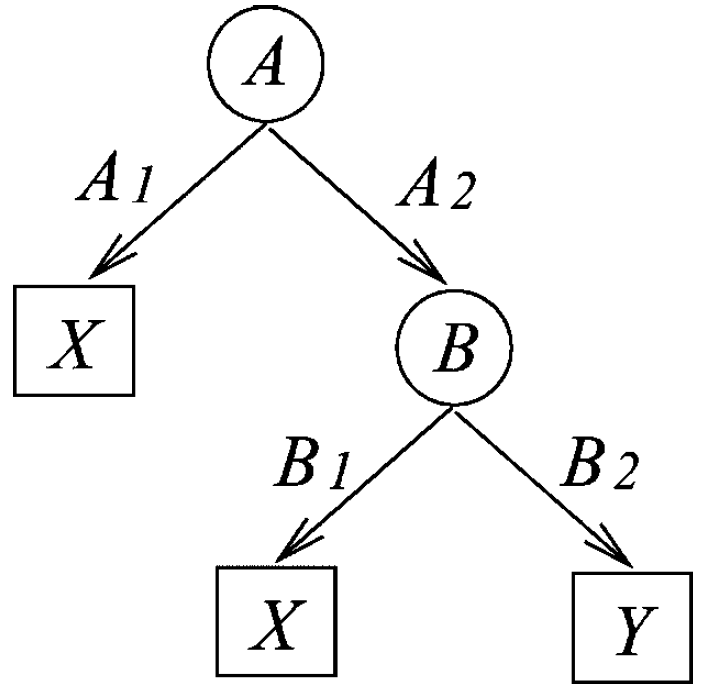
\includegraphics[width=\textwidth]{figures/FDTvsFPT_FDT}
%                \caption{Árvore de decisão \emph{Fuzzy}}
%                \label{Fig:FDTvsFPT_FDT}
%        \end{subfigure}%
%        \hspace{6em} %add desired spacing between images, e. g. ~, \quad, \qquad, \hfill etc.
%          %(or a blank line to force the subfigure onto a new line)
%        \begin{subfigure}[t]{0.3\textwidth}
%                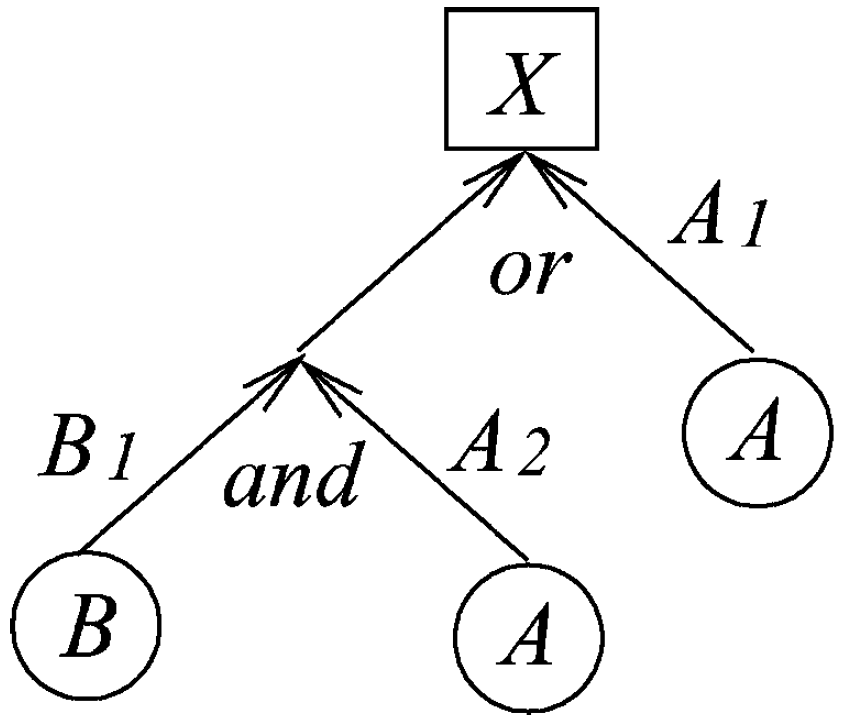
\includegraphics[width=\textwidth]{figures/FDTvsFPT_FPT}
%                \caption{\emph{Fuzzy Pattern Tree}}
%                \label{Fig:FDTvsFPT_FPT}
%        \end{subfigure}
%        \caption{Exemplos de árvores construídas a partir de um mesmo conjunto de exemplos \cite{Huang2008}}\label{Fig:FDTvsFPT}
%\end{figure}
%
%A proposta apresentada em \cite{Shaker2013} é um método de classificação adaptativo baseado na indução de \emph{Fuzzy Pattern Trees}. Esta proposta implementa um mecanismo de adaptação que identifica, de forma preditiva, possíveis mudanças locais no modelo atual. A ideia básica do método é manter um conjunto de \emph{Fuzzy Pattern Trees} composto pelo modelo atual (ativo) e um conjunto de modelos vizinhos. A predição é realizada pelo modelo ativo, enquanto os modelos vizinhos funcionam como adaptações antecipadas. Os modelos vizinhos são mantidos até que a performance do modelo ativo tenha queda significativa, causada, por exemplo, por um desvio de conceito. Neste momento, o modelo atual é substituído pelo modelo vizinho mais adequado.
%
%\citeonline{Wang2013} expõem a proposta de um \emph{framework} geral para a utilização de pesos \emph{fuzzy} para cada exemplo do FD. De forma incremental, conforme a chegada de novos exemplos, o cálculo da pertinência, baseado na informação de rótulo, é efetuado, levando em conta as pertinências já calculados para exemplos antigos. O cálculo de distância proposto e utilizado no trabalho, que é baseado na descoberta de centróides de classe e distância entre pares de exemplos, pode colaborar para a identificação de possíveis \emph{outliers}. A priori, o \emph{framework} pode ser utilizado em conjunto com qualquer algoritmo de classificação que faça uso da informação obtida na forma de pesos. Os autores optaram por vincular, de forma direta, um algoritmo baseado em redes neurais, o \emph{Passive-Agressive} (PA) \cite{Crammer2006}, constituindo a técnica neuro-\emph{fuzzy} \cite{Jang1997} chamada de \emph{Fuzzy Passive-Agressive}.
%
%%\undecided{\subsection{Aprendizado Supervisionado em FD baseado em \emph{Ensemble} de Classificadores}}
%
%A ideia da construção de um modelo preditivo pela integração de múltiplos modelos \cite{Witten2005,Rokach2010} também pode ser encontrada no aprendizado em FD. Abordagens que se utilizam deste sistema serão tratadas, doravante, pelo termo geral \emph{Ensemble} de Classificadores (EC).
%
%\citeonline{Tsymbal2008} propõe uma técnica de integração dinâmica de EC para auxiliar no trabalho de identificação e tratamento de desvios de conceito, onde cada classificador recebe um peso proporcional a sua acurácia local. Para a classificação final, o melhor classificador base, quando houver, é selecionado ou é realizada uma votação ponderada entre os classificadores.
%
%Desvios de conceitos e contexto é o foco no trabalho de \citeonline{Gomes2011}. A proposta baseada em EC realiza a detecção de mudanças de conceito e, dinamicamente, adiciona e remove classificadores ponderados de acordo com o que foi identificado. Conceitos estáveis são detectados por método baseado na taxa de erro do processo de aprendizado. A informação de contexto é utilizada na adaptação a conceitos recorrentes (ou ressurgentes) e no gerenciamento de conhecimento aprendido previamente.
%
%%\undecided{\subsection{Other ?}}
%
%A dificuldade de classificação de instâncias incompletas também é uma preocupação quando tratamos de aprendizado em FD. A maior parte das abordagens assume que todos os exemplos do FD possuem valores para um determinado conjunto de atributos, no entanto existem esforços \cite{MillanGiraldo2011} para que os exemplos sem um ou mais atributos possam ser aproveitados no processo de aprendizagem. 
%
%Pesquisadores têm investido na área de classificação em FD, porém é importante ressaltar que nem sempre existem rótulos disponíveis para realizar esse tipo de tarefa de aprendizado e a rotulação manual dos exemplos de um FD é inviável considerando seu tamanho potencialmente infinito. A próxima seção descreve técnicas de agrupamento em FD. 

%\section{Técnicas de Aprendizado Semissupervisionado em Fluxos de Dados}

A busca por melhores resultados no aprendizado em FD impulsionou o desenvolvimento de técnicas semissupervisionadas para trabalhar neste contexto. As abordagens de aprendizado semissupervisionado para conjuntos estáticos, juntamente com as abordagens de aprendizado supervisionado e não supervisionado em FD servem de inspiração para as propostas descritas nas próximas seções.

\section{Classificação Semissupervisionada em FD}

As técnicas de aprendizado semissupervisionado baseadas em classificadores assumem que o conjunto de dados é parcialmente rotulado. No caso desse tipo de aprendizado em FD, a parte rotulada dos exemplos pode ser apenas um pequeno conjunto que irá gerar o modelo inicial de classificação ou é possível encontrar exemplos rotulados no próprio fluxo.

Considerando essas duas situações de disponibilidade de rótulos, podem ser encontradas na literatura propostas baseadas em diferentes métodos de classificação, por exemplo: redes neurais \cite{Leite2010,Astudillo2011,Astudillo2013,Bouguelia2013,Kasabov2013}, baseada em grafos \cite{Tiwari2010,Bertini2012,Bertini2013}, competição de partículas \cite{Breve2012,Breve2013}, SVM \cite{Frandina2013}, entre outros \cite{Pan2007,FdezRiverola2007,DeSilva2011}.

Uma proposta \cite{Liang2012} baseada em CVFDT considera que o FD possui rótulo positivo e os dados incertos são não rotulados, realizando o aprendizado de forma semissupervisionada.

Técnicas baseadas em \emph{ensemble} de classificadores também são populares no aprendizado semissupervisionado em FD. \citeonline{Kholghi2011} apresentam uma proposta para um \emph{framework} que combina semissupervisão por meio de \emph{Active Learning} \cite{Settles2010} e a consideração da influência de exemplos não rotulados a fim de melhorar a performance de aprendizagem. Um modelo é construído para predição de rótulos de exemplo futuros com alto valor de acurácia. Esse modelo de predição é baseado em um \emph{ensemble} de classificadores construídos a partir de \emph{chunks} de exemplos do FD. Esta é uma das primeiras tentativas de incorporação de \emph{Active Learning} semissupervisionado em FD.

\section{Agrupamento Semissupervisionado em FD}

No aprendizado semissupervisionado baseado em agrupamento, considera-se conhecimento prévio durante o processo de agrupamento para melhorar o aprendizado. Esta informação pode estar disponível em diferentes formas, por exemplo rótulos para parte do FD, restrições entre pares de exemplos, informações estatísticas sobre a distribuição dos exemplos.

Quando há uma pequena quantidade de exemplos rotulados disponíveis, estes podem ser utilizados como sementes que contribuirão para guiar o algoritmo de agrupamento. O modelo de \emph{flocking} serve de inspiração para a adaptação de um algoritmo de agrupamento para aprendizado em FD \cite{Bruneau2009}, utilizando um pequeno conjunto de dados rotulados como informação para um operador de divisão de um grupo de exemplos, que permite a adaptação do agrupamento a mudanças no FD.

Uma técnica de agrupamento semissupervisionado baseada em AP \cite{Shi2009} utiliza informação prévia na forma de rótulos no ajuste da matriz de similaridade do modelo produzido e promove um estudo para ampliar o conjunto de dados rotulados. Baseado em \emph{Fuzzy Pattern Matching} \cite{Cayrol1982,Dubois1988}, o método proposto em \cite{Mouchaweh2010} tem o objetivo de aprender funções de pertinência com um conjunto de exemplos rotulados inicial limitado. A função de pertinência das classes é aprendida e atualizada, de acordo com a chegada de novos exemplos com rótulos.

O algoritmo \emph{Compound Gaussian Mixture Model} \cite{Gao2010}, baseado no agrupamento \emph{Gaussian Mixture Model}, utiliza amostra de dados rotulados em uma fase que aplica uma extensão do algoritmo \emph{Expectation Maximization} \cite{Zhou2007} para melhorar o agrupamento. A técnica \emph{Growing Type-2 Fuzzy Classifier} \cite{Bouchachia2014} utiliza uma versão \emph{online} do agrupamento \emph{Gaussian Mixture Model} para gerar partições \emph{fuzzy} tipo-2 \cite{Mendel2002} para construir regras de classificação, empregando conjunto parcialmente rotulado no aprendizado. Esta técnica possui mecanismos para aprendizado em FD.

\citeonline{Atwa2014} propõem um algoritmo de agrupamento semissupervisionado que extende o AP para lidar com FD. Um conjunto de instâncias rotuladas é incorporado para detecção de mudança, que requer a atualização do modelo o mais rápido possível. 

Em um contexto de FD com multirrótulos, o \emph{Hierarchical Semi-supervised Impurity based Subspace Clustering} \cite{Ahmed2010} captura a correlação implícita existente entre cada par de rótulos de classe.

Técnicas que utilizam informação na forma de restrições podem obtê-las a partir de exemplos rotulados, mas também pode ser um conhecimento pré-existente nesse formato. O \emph{C-DenStream} \cite{Ruiz2009} é uma técnica baseada no algoritmo \emph{DenStream} adaptado para a utilização o conceito de restrições entre pares de exemplos estendido para FD. O \emph{C-DenStream} foi uma das primeiras extensões do paradigma de aprendizado por agrupamento semissupervisionado estático para FD e, embora traga ganhos nesse contexto, ainda possui as limitações do \emph{DenStream}. 

\citeonline{Halkidi2012} utiliza, além do FD, um fluxo contínuo de restrições, introduzindo o conceito de multigrupos (regiões densas e sobrepostas) e implementa mecanismo para identificação de \emph{outlier}. \citeonline{Sirampuj2013} \label{chRevisao:Sirampuj2013} propõem um algoritmo para agrupamento em FD também com uso de conhecimento prévio na forma de restrições. A técnica, que é uma extensão do \emph{E-Stream} \cite{Udommanetanakit2007} possui mecanismos para lidar com restrições que mudam de acordo com o tempo (técnica de esquecimento).

\citeonline{Cheng2011} desenvolvem um \emph{framework} para análise de agrupamento de textos e desenvolvimento de um novo modelo de agrupamento semissupervisionado, capaz de lidar com informação prévia na forma de restrições entre pares de exemplos e rótulos de maneira simultânea.

Uma proposta de método para agrupamento em FD incertos (domínios onde há ruído e dados incompletos) \cite{Aggarwal2008} utiliza um modelo geral de incerteza, no qual assume-se que algumas estatísticas de incerteza estão disponíveis. 

\section{Aprendizado Semissupervisionado Híbrido em FD}

É possível identificar dentro do aprendizado semissupervisionado algumas abordagens híbridas, ou seja, inspiradas em métodos de agrupamento e classificação trabalhando em conjunto para melhorar o aprendizado.

\citeonline{Wu2009} apresentam um método semissupervisionado para a construção de um rastreador de tópicos (\emph{topical crawler}), aplicando um agrupamento $k$-\emph{means} com restrições entre pares para detectar novas amostras de páginas enviadas a um classificador de páginas e preditor de links para atualização de modelos aprendidos.

A proposta de \citeonline{Borchani2011} é a combinação do método de \cite{Dasu2006} adaptado em um algoritmo de agrupamento para aprendizado semissupervisionado. O algoritmo de agrupamento é utilizado para atualização do modelo quando ocorre desvio de conceito.

Técnicas baseadas em AH podem utilizar métodos de agrupamento para divisão e rotulação em suas folhas. \citeonline{Li2012} estende trabalho anterior \cite{Li2010} e propõem um algoritmo de classificação semissupervisionada em FD, utilizando uma árvore de decisão como modelo de classificação. Para o crescimento da árvore, utiliza-se de um algoritmo de agrupamento baseado no $k$-\emph{means} para a produção de grupos de conceito e rotulação automática de dados não rotulados. Potenciais desvios de conceito são identificados e conceitos recorrentes são mantidos. Uma técnica semelhante considera informação prévia na forma de rótulos e aplica uma versão semissupervisionada do algoritmo de agrupamento $k$-\emph{modes} para produzir grupos de conceito \cite{Li2010a,wu2012}.

\emph{Clustering Feature Decision Tree} \cite{Xu2011} realiza a construção de uma árvore de decisão a partir de FD parcialmente rotulados, aplicando algoritmo de agrupamento para gerar um vetor de atributos de grupos, sumários estatísticos que serão usados para indução da árvore de decisão. Os vetores de grupos também são empregados na classificação de exemplos nas folhas da árvore.

\citeonline{Zhang2009} propõem um \emph{framework} para construção de modelos a partir de FD com exemplos rotulados e não rotulados. Para a construção do modelo, os dados do FD são associados a quatro categorias distintas, cada qual correspondendo à situação de desvio de conceito, podendo existir ou não nos exemplos rotulados e não rotulados. Em seguida, é aplicado método de aprendizado SVM semissupervisionado baseado no $k$-\emph{means}.

A técnica \emph{Concurrent Semi-supervised Learning of Data Streams} \cite{Nguyen2011,Nguyen2013} aplica o potencial de aprendizado semissupervisionado concorrente, onde um modelo de agrupamento e um de classificação são construídos de forma simultânea e colaborativa, fazendo uso de um pequeno conjunto de exemplos rotulados encontrados em um FD.

Outras propostas utilizam aprendizado semissupervisionado com objetivo de apenas estender o conjunto de exemplos rotulados e, então, aplicar método de aprendizado supervisionado com mecanismos disponíveis para lidar com as particularidades de FD. \citeonline{Wu2006} coloca a proposta de um algoritmo de aprendizado semissupervisionado baseado em treinamento por agrupamento, para seleção de exemplos confiáveis a serem rotulados e utilizados no retreinamento de um classificador. A técnica proposta por \cite{Yu2009} aplica um algoritmo de agrupamento semissupervisionado aos exemplos parcialmente rotulados do FD na tentativa de estender o conjunto de exemplos rotulados, utilizando-os para atualização de um modelo supervisionado que conta com mecanismos de esquecimento.

O \emph{framework} \emph{COMPOSE} \cite{Dyer2014} aprende desvios de conceitos em ambiente de FD onde há apenas um conjunto inicial de dados rotulados e, após a inicialização, apenas dados não rotulados. O \emph{COMPOSE} segue três passos:
\begin{enumerate*}[label=\itshape\arabic*\upshape)]
\item combinação dos dados rotulados iniciais aos dados não rotulados atuais para treinar um classificador semissupervisionado e rotular de forma automática o conjunto de dados;
\item para cada classe, construção de formas que englobam os exemplos, representando a distribuição atual da classe;
\item compactação das formas e extração de instâncias representantes (\emph{core supports}), que servirão como conjunto rotulado inicial para os próximos novos dados não rotulados
\end{enumerate*}.

\section{\emph{Ensemble} de Modelos para Aprendizado Semissupervisionado em FD}

Algumas propostas para aprendizado semissupervisionado em FD tem a intenção de aproveitar da construção de diversos modelos trabalhando em conjunto para melhorar a representação dos exemplos do FD.

O trabalho apresentado em \cite{Zhang2012} é uma adaptação do trabalho \cite{Zhang2009}, onde para cada categoria de exemplo de treinamento é construído um modelo distinto para classificação, baseado em SVM. Em \cite{Zhang2014a} os modelos base para o \emph{ensemble} são construídos por método de aprendizado semissupervisionado, utilizando conjunto de exemplos rotulados e não rotulados. Informação histórica é mantida como parte de peso no fator de decisão para classificação de novos exemplos.

O trabalho de \citeonline{Nahar2014a} propõe um \emph{framework} para detecção de \emph{cyberbullying} utilizando um classificador \emph{ensemble} semissupervisionado. Em outra proposta \cite{Nahar2014}, a técnica utiliza inclui a extensão do conjunto de dados rotulados por meio de um classificador \emph{ensemble}, com aplicação de um algoritmo \emph{fuzzy} SVM para ponderar o espaço de atributos do domínio.

Outras técnicas têm a extensão do conjunto de exemplos rotulados como parte do processo de aprendizado semissupervisionado. \citeonline{Cao2008} apresenta um algoritmo iterativo que recupera rótulos de acordo com níveis de confiança para melhorar o sistema aprendido pela geração de vários modelos de classificação. A técnica utilizada por \citeonline{Ahmadi2012} treina classificadores usando os exemplos rotulados e tenta classificar os exemplos não rotulados por meio do \emph{ensemble} para estender o conjunto de treinamento e adaptar os modelos de classificação.

O trabalho \cite{Masud2008} descreve uma proposta baseada na construção de microgrupos pela aplicação de método de agrupamento semissupervisionado e construção de classificadores pelo algoritmo $K$-\emph{Nearest Neighbors} para cada\emph{chunk} de exemplos do FD. Os $L$ melhores modelos (de acordo com acurácia individual) são utilizados em um \emph{ensemble}.

A proposta de \citeonline{Ditzler2011} apresenta um \emph{ensemble} onde classificadores são treinados a partir dos exemplos rotulados do FD. Omodelo de classificação utiliza pesos para determinar a influência de cada classificador na decisão final e esses pesos são determinadospeladistância entre componentes de um \emph{Gaussian Mixture Model} treinado com o conjunto completo de exemplos.

\citeonline{Masud2012} propõem um \emph{ensemble} onde cada modelo de classificação é construindo como uma coleção de microgrupos, usando agrupamento semissupervisionado, e exemplos não rotulados são classificados de acordo com o conjunto de modelos. 

Uma proposta \cite{Liu2013} mantém um \emph{ensemble} de modelos mistos, baseados em métodos de classificação e agrupamento. Os exemplos rotulados são utilizados para treinamento de classificador supervisionado e novos exemplos rotulados são empregados na atualização desse classificador. Os exemplos não rotulados são utilizados na construção de modelos não supervisionado. O \emph{ensemble} segue um modelo semissupervisionado de classificação de forma a maximizar o consenso entre os diferentes modelos.

\section{Considerações Finais}

Neste capítulo foram colocadas algumas técnicas de aprendizado em FD. A maioria das propostas sugere adaptações para métodos de aprendizado em conjuntos estáticos, a fim de incluir mecanismos que possam lidar com as limitações de aprendizado em FD.

Recentemente, percebe-se uma preocupação em elaborar técnicas que possam realizar o aprendizado de forma semissupervisionada, uma vez que a maior parte dos domínios não possuem uma quantidade grande de rótulos. O modelo supervisionado aprendido apenas pelo pequeno conjunto de exemplos rotulados pode ser ineficiente, enquanto modelos aprendidos de forma não supervisionada perdem a chance de melhorar o resultado pela consideração de informação prévia sobre o FD.

As técnicas apresentadas neste capítulo utilizam métodos variados de aprendizado de máquina e implementam diferentes mecanismos para atacar os problemas característicos de aprendizado em FD. Alguns trabalhos sugerem adaptações e extensões para melhorar um ou outro aspecto de um método. De forma geral, a forma de como lidar com o tempo (mecanismos de esquecimento) e detecção de desvio de conceitos são duas tarefas relevantes que não são consideradas por todas as técnicas de aprendizado em FD. De qualquer forma, a revisão colocada no capítulo contribui para uma visão geral do estado da arte quanto ao aprendizado em FD.

O \autoref{chProposta} discute a proposta de trabalho para elaboração da tese de doutorado dentro do tema de aprendizado de máquina semissupervisionado em FD.

%\input{Chapter/algoritmos}

% ----------------------------------------------------------
% PARTE - Proposta
% ----------------------------------------------------------
\part{Proposta, Experimentos e Resultados}

\chapter{Proposta} \label{chProposta}

\rewrite{
Dificuldade de generalizar técnicas \emph{crisp} de agrupamento em fluxo de dados para técnicas \emph{fuzzy} \cite{Hore2007}

Maior parte das abordagens utiliza protótipos ponderados como estrutura de sumarização. Processa os dados em chunks.

\begin{itemize}
    \item Uma das dificuldades nessa estratégia é determinar o valor de $h$, uma vez que essa definição depende do domínio ao qual é aplicado o agrupamento.
    
    \item Outra complicação de estratégias baseadas no SPFCM é a definição prévia de um número fixo de grupos, pois, uma vez que um FD é mutável de acordo com o tempo pode ocorrer o aumento ou diminuição no número de grupos. Outro obstáculo: identificação de grupos de formato arbitrário (?)
\end{itemize}
}
\chapter{Experimentos} \label{ChExp}
\section{Conjuntos de Dados}

\subsection{Sintéticos}

\subsubsection*{Estacionários}

Estáticos 2D \autoref{Fig:SinteticosEstaticos}.

set.seed(1000)

gerador R: Barras e Gaussianas com 10000 exemplos - A data stream generator which creates the shape of two bars and two Gaussians clusters with different density. Conjunto BG\_10k, \autoref{Fig:BarGauss}.

gerador R: Mistura de Gaussianas - A data stream generator that produces a data stream with a mixture of static Gaussians

3 Gaussianas em 2 dimensões com 10000 exemplos. Conjunto MGK3D2\_10k, \autoref{Fig:GaussK3D2}.

4 Gaussianas em 2 dimensões com 10000 exemplos. Conjunto MGK4D2\_10k, \autoref{Fig:GaussK4D2}.

\begin{figure}[!htb]
        \centering
        \begin{subfigure}[t]{0.4\textwidth}
                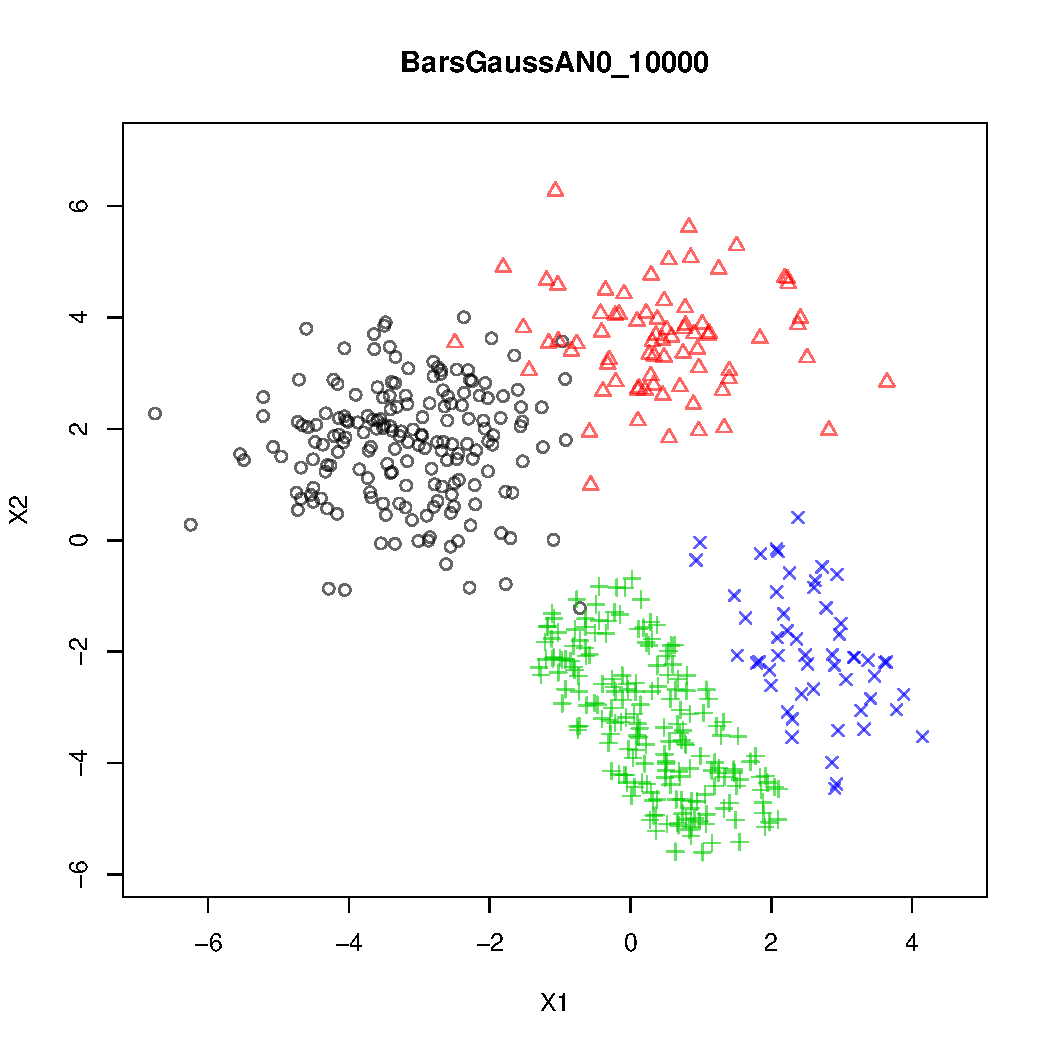
\includegraphics[width=\textwidth]{figures/datasets/BarsGaussAN0_10000}
                \caption{BG\_10k}
                \label{Fig:BarGauss}
        \end{subfigure}%
        \qquad %add desired spacing between images, e. g. ~, \quad, \qquad, \hfill etc.
          %(or a blank line to force the subfigure onto a new line)
        \begin{subfigure}[t]{0.4\textwidth}
                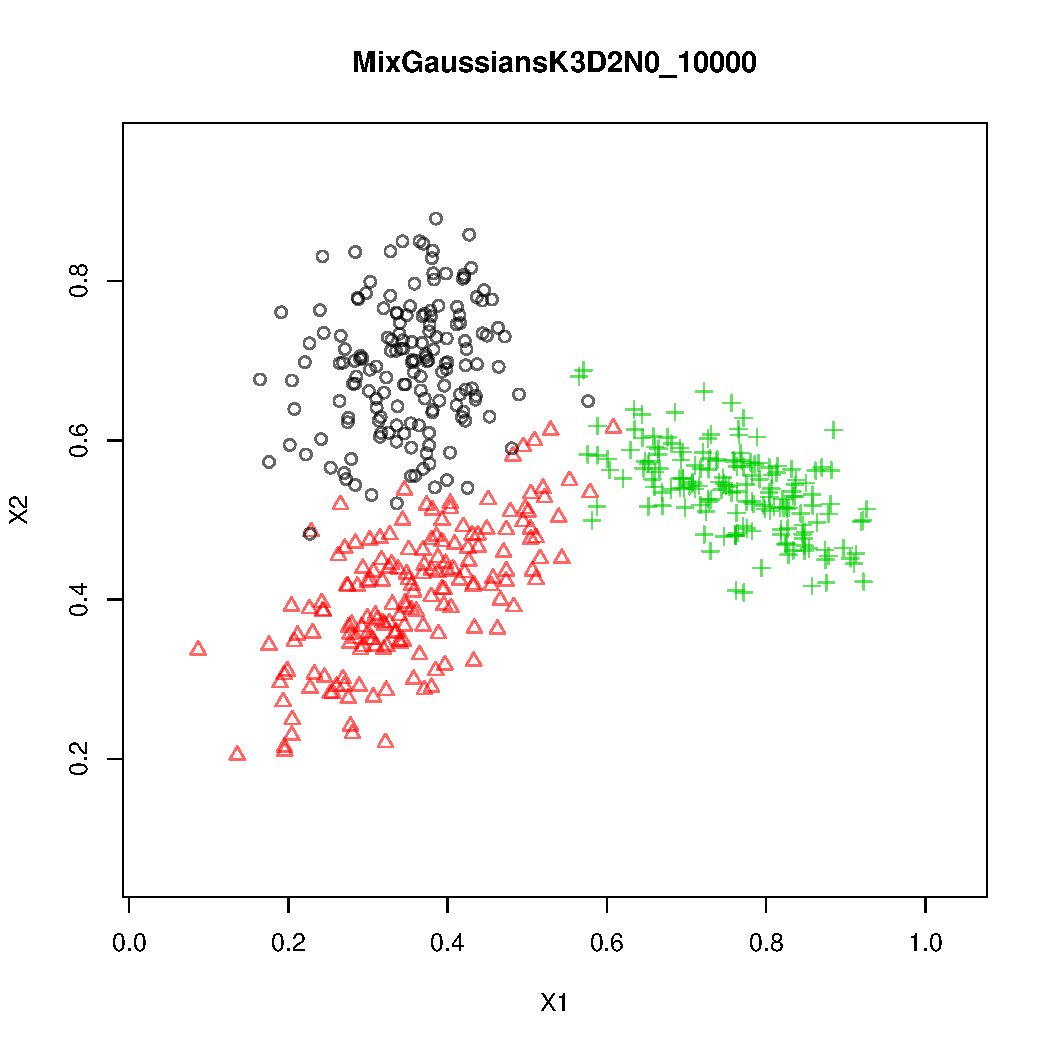
\includegraphics[width=\textwidth]{figures/datasets/MixGaussiansK3D2N0_10000}
                \caption{MGK3D2\_10k}
                \label{Fig:GaussK3D2}
        \end{subfigure}
        \qquad %add desired spacing between images, e. g. ~, \quad, \qquad, \hfill etc.
        %(or a blank line to force the subfigure onto a new line)
        \begin{subfigure}[t]{0.4\textwidth}
                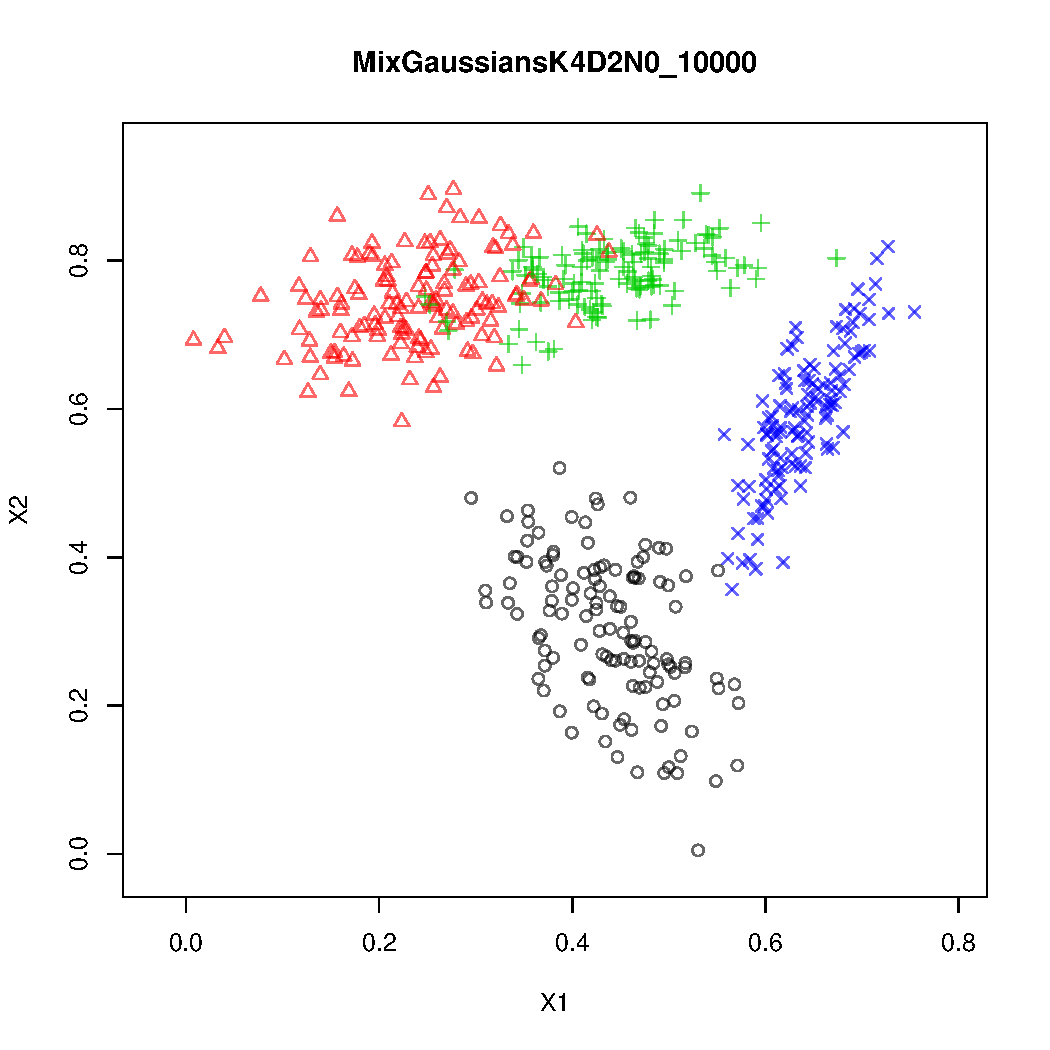
\includegraphics[width=\textwidth]{figures/datasets/MixGaussiansK4D2N0_10000}
                \caption{MGK4D2\_10k}
                \label{Fig:GaussK4D2}
        \end{subfigure}
        \caption{Gráficos 500 pares de exemplos de cada conjunto BG\_10k, MGK3D2\_10k e MGK4D2\_10k}\label{Fig:SinteticosEstaticos}
\end{figure}

Mistura de 3 Gaussianas em 3 dimensões com 10000 exemplos. Conjunto MGK3D3\_10k, \autoref{Fig:GaussK3D3}.

\subsubsection*{Não Estacionários}

gerador R: DSD\_Benchmark(i) - A data stream generator that generates several dynamic streams indented to be benchmarks to compare data stream clustering algorithms. Available: $i = 1$ e $i = 2$.

DSD\_Benchmark(1) - creates two clusters moving in two-dimensional space. One moves from top left to bottom right and the other one moves from bottom left to top right. Both clusters overlap when they meet exactly in the center of the data space.

Com 5500 exemplos. Conjunto GB1\_5.5k \autoref{Fig:Benchmark1}.

\begin{figure}[!htb]
        \centering
        \begin{subfigure}[t]{0.25\textwidth}
                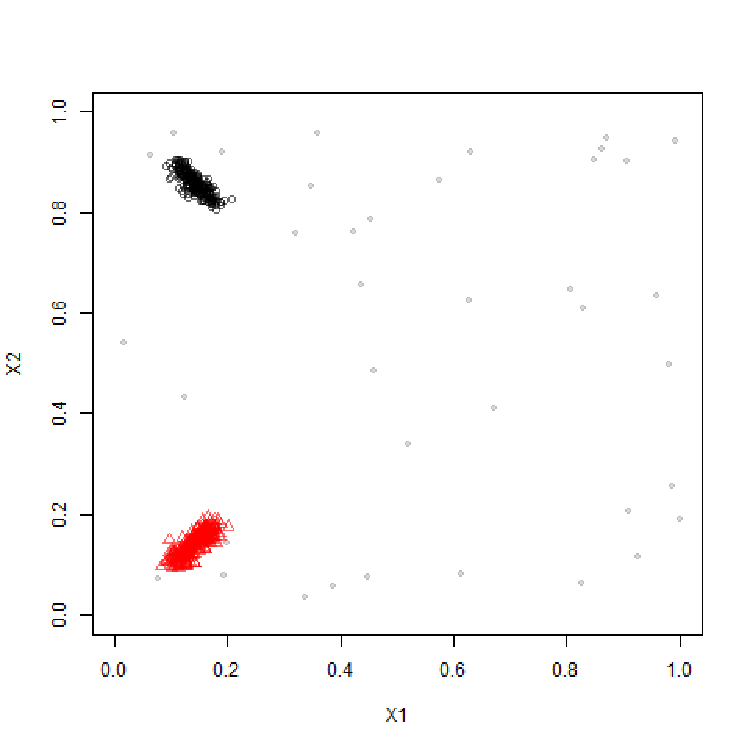
\includegraphics[page=1,width=\textwidth]{figures/datasets/Benchmark1_5500}
                \caption{$t = 0$}
                \label{Fig:Benchmark1_11}
        \end{subfigure}%
        \qquad %add desired spacing between images, e. g. ~, \quad, \qquad, \hfill etc.
          %(or a blank line to force the subfigure onto a new line)
%        \begin{subfigure}[t]{0.25\textwidth}
%                \includegraphics[page=3,width=\textwidth]{figures/datasets/Benchmark1_5500}
%                \caption{$t = 2$}
%                \label{Fig:Benchmark1_12}
%        \end{subfigure}%
%        \qquad %add desired spacing between images, e. g. ~, \quad, \qquad, \hfill etc.
        %(or a blank line to force the subfigure onto a new line)
        \begin{subfigure}[t]{0.25\textwidth}
                \includegraphics[page=5,width=\textwidth]{figures/datasets/Benchmark1_5500}
                \caption{$t = 4$}
                \label{Fig:Benchmark1_13}
        \end{subfigure}%
		\qquad %add desired spacing between images, e. g. ~, \quad, \qquad, \hfill etc.
        %(or a blank line to force the subfigure onto a new line)
        \begin{subfigure}[t]{0.25\textwidth}
                \includegraphics[page=6,width=\textwidth]{figures/datasets/Benchmark1_5500}
                \caption{$t = 5$}
                \label{Fig:Benchmark1_14}
        \end{subfigure}%
		\qquad %add desired spacing between images, e. g. ~, \quad, \qquad, \hfill etc.
        %(or a blank line to force the subfigure onto a new line)
        \begin{subfigure}[t]{0.25\textwidth}
                \includegraphics[page=7,width=\textwidth]{figures/datasets/Benchmark1_5500}
                \caption{$t = 6$}
                \label{Fig:Benchmark1_15}
        \end{subfigure}%
        \qquad %add desired spacing between images, e. g. ~, \quad, \qquad, \hfill etc.
        %(or a blank line to force the subfigure onto a new line)
%        \begin{subfigure}[t]{0.25\textwidth}
%                \includegraphics[page=9,width=\textwidth]{figures/datasets/Benchmark1_5500}
%                \caption{$t = 8$}
%                \label{Fig:Benchmark1_16}
%        \end{subfigure}%
%		\qquad %add desired spacing between images, e. g. ~, \quad, \qquad, \hfill etc.
        %(or a blank line to force the subfigure onto a new line)
        \begin{subfigure}[t]{0.25\textwidth}
                \includegraphics[page=11,width=\textwidth]{figures/datasets/Benchmark1_5500}
                \caption{$t = 10$}
                \label{Fig:Benchmark1_17}
        \end{subfigure}%
		\caption{500 exemplos do conjunto GB1\_5.5k em diferentes tempos $t$}\label{Fig:Benchmark1}
\end{figure}

\rewrite{
Benchmark1 com 11000 exemplos (vai e volta) - se eu conseguir rodar

DSD\_Benchmark(2) - ver qual o comportamento

DSD\_MG, a generator to specify complex data streams with concept drift. The shape as well as the behavior of each cluster over time (changes in position, density and dispersion) can be specified using keyframes (similar to keyframes in animation and film making) or by mathematical functions.

DSD\_RandomRBFGeneratorEvents (streamMOA) generates streams using radial base functions with noise. Clusters move, merge and split.
}

\subsection{Benchmark}

\begin{itemize}
    \item KDDCup 99
    \item Forest Covertype
\end{itemize}
\section{Ferramentas}

Com o crescimento da pesquisa sobre aprendizado em FD, é interessante o investimento em ferramenta de software para a aplicação das diversas técnicas propostas. Existem hoje ferramentas, disponíveis gratuitamente, como:

\begin{itemize}
    \item \textbf{MOA (\emph{Massive On-line Analysis}} \cite{MOA} - um \emph{framework} de código aberto que disponibiliza implementação de uma série de algoritmos e métricas para classificação, principalmente, e para agrupamento em FD. A ferramenta também conta com recursos para visualização dos processos de aprendizado.
    
    \item \textbf{VFML (\emph{Very Fast Machine Learning})} \cite{VFML} - um pacote de implementações para mineração de FD de alta velocidade e conjuntos de exemplos \emph{very large}.% Está disponível pelo endereço: http://www.cs.washington.edu/dm/vfml/.
\end{itemize}

A linguagem R \cite{linguagemR} vem sendo muito utilizada para análise de dados e aprendizado de máquina, ... Foi escolhida para implementação da proposta e execução de experimentos.

O pacote \textbf{stream} \cite{lingR_Stream} ... R

O pacote \textbf{streamMOA} \cite{lingR_StreamMOA} ...  interface java moa  -- R

O pacote \textbf{e1071} \cite{lingR_e1071} ... FCM

\section{Técnicas de Agrupamento em Fluxos de Dados}

\rewrite{apresentar de outra forma (tabela?), destacar mais relevantes/importantes?}

Abordagens de agrupamento de dados são tipicamente utilizadas no aprendizado não supervisionado. Dentro da área de FD é comum verificar a falta de informação de classe, seja por conta da natureza do domínio (não existem classes definidas) ou pela dificuldade em rotular exemplos de um FD.

Independentemente dos métodos adotados, é desejável que algoritmos de agrupamento em FDs possuam a capacidade de \cite{Amini2014}: 
\begin{enumerate*}[label=\itshape\alph*\upshape)]
\item descobrir grupos de formatos arbitrários;
\item lidar com ruído;
\item realizar o agrupamento sem informação prévia sobre o número de grupos
\end{enumerate*}.

%Há diferentes técnicas para agrupamento em FD e elas podem ser divididas de acordo com a abordagem de agrupamento que seguem.

\rewrite{falar sobre propostas baseada em chunks de exemplos}

\subsection{\emph{Framework Online-Offline} (FOO) para Agrupamento em FD} \label{ChAFD:framework}

Algoritmos de agrupamento baseados em exemplos podem ser resumidos em dois passos \cite{Cao2006,Yang2006}: abstração dos dados (componente\emph{online}) e agrupamento (componente \emph{offline}), ilustrados na \autoref{Fig:onlineOffline}.

\begin{figure}[!htb]
	\centering
	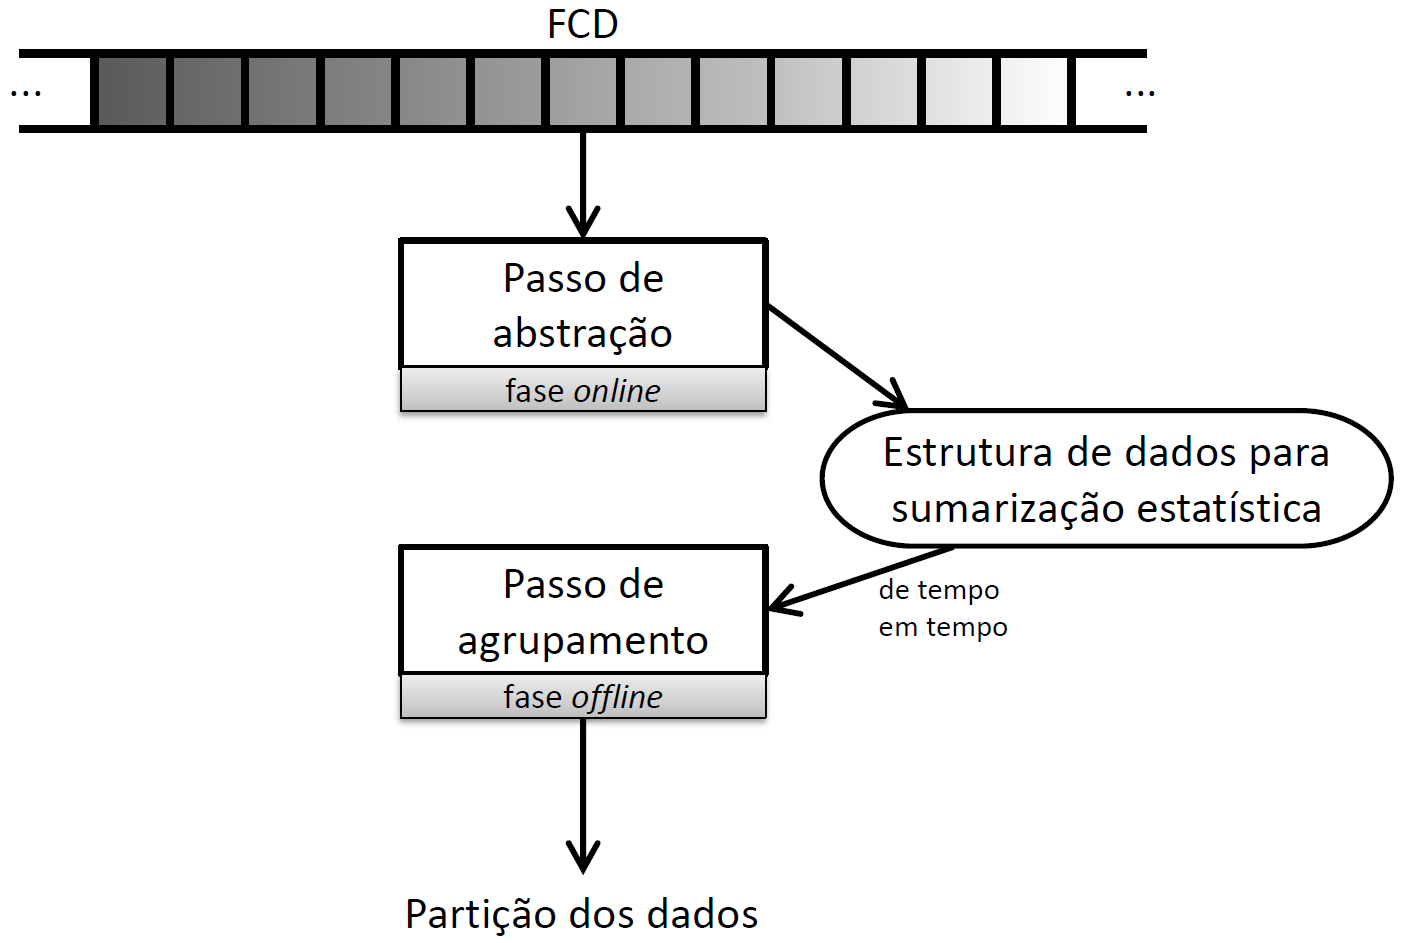
\includegraphics[width=0.7\textwidth]{figures/onlineOffline}
	\caption{\emph{Framework} \emph{online-offline} \cite{Silva2013}}\label{Fig:onlineOffline}
\end{figure}

A fase \emph{online}, abstração dos dados, sumariza os dados do FD com o auxílio de estruturas particulares para lidar com restrições de espaço e memória das aplicações FD. Essas estruturas de sumarizam os dados para preservar o significado dos objetos originais sem a necessidade de armazená-los. Estruturas frequentemente utilizadas são vetores de atributos, arranjos de protótipos e grades de dados. Essas estruturas são melhor detalhadas na \autoref{chConceitos:FD:Sumario}.

Para a contínua sumarização dos exemplos que chegam e dar maior importância aos exemplos mais recentes, uma abordagem popular é a definição de janelas temporais, como apresentado na \autoref{chConceitos:FD:Janelas}.

Durante o passo de abstração, algoritmos de agrupamento em FD devem utilizar mecanismos para detecção de \emph{outliers} que sejam capazes de diferenciar verdadeiros \emph{outliers} de evolução de grupos (\autoref{chConceitos:FD:Desvios}), uma vez que a distribuição dos dados pode variar de acordo com o tempo.

Na fase \emph{offline} é possível obter uma partição dos dados pelo passo de agrupamento. Neste momento, pode ser necessária a definição de alguns valores de entrada (número de grupos, por exemplo) para que seja possível ter uma visão geral dos grupos do FD. Algoritmos de agrupamento tradicionais podem ser utilizados considerando o conjunto de estruturas de sumarização para encontrar uma partição dos dados. O formato dos grupos encontrados está ligado ao algoritmo de agrupamento empregado, por exemplo, o $k$-\emph{means} \cite{macqueen1967} gera grupos hiperesféricos enquanto o DBSCAN \cite{Ester1996} é capaz de descobrir grupos de formatos aleatórios.

O \emph{framework} apresentado nesta seção é frequentemente utilizado para o desenvolvimento de novas técnicas de agrupamento em FD. Algumas dessas propostas são discutidas no \autoref{ChSemi}.

O \emph{ClusTree} \cite{Kranen2011}, por exemplo, é a proposta de uma estrutura hierárquica compacta e auto-adaptativa para manter sumários de FD, construindo uma hierarquia de microgrupos em diferentes níveis. Outras técnicas que seguem a abordagem hierárquica de agrupamento são o \emph{E-Stream} \cite{Udommanetanakit2007}, que possui suporte para cinco tipos de evolução em grupos (aparecimento, desaparecimento, evolução própria, mescla e divisão), e suas extensões para suporte de incerteza (valores faltantes) em FDs heterogêneos (conjuntos que combinam atributos numérico-contínuos e categóricos) \cite{Meesuksabai2011} e FDs de alta dimensão \cite{Chairukwattana2014}.

As subseções a seguir apresentam técnicas já existentes baseadas em agrupamento particional e baseado em densidade, onde é possível identificar focos de pesquisas mais recentes.

\subsection{Agrupamento Particional em FD}

Os algoritmos de agrupamento particional para FD, em sua maioria, são propostos como extensões de algoritmos de agrupamento particionais conhecidos, como $k$-\emph{means}, $k$-medóides e \emph{Affinity Propagation}.

O algoritmo \emph{CluStream} \cite{Aggarwal2003} é baseado no algoritmo $k$-\emph{means} e introduz um \emph{framework} \emph{online-offline} para agrupamento em FD que vem sendo adotado para grande parte dos algoritmos propostos recentemente. \citeonline{Yang2006} propõem uma extensão chamada \emph{HCluStream} para lidar com FDs heterogêneos.

A proposta de \citeonline{Labroche2014} está baseada no algoritmo $k$-medóides e realiza agrupamento \emph{fuzzy} de forma incremental. O trabalho de \citeonline{Lemos2013} apresenta uma técnica para geração de um classificador \emph{fuzzy} baseado em agrupamento incremental para a geração de regras que descrevem novos estados operacionais de um sistema de detecção e diagnóstico de falhas.

\citeonline{Hore2007} apresentam a proposta de uma abordagem genérica para agrupamento iterativo \emph{fuzzy}/possibilístico em FD, introduzindo equações objetivo transformadas para os algoritmo FCM \cite{Bezdek1981}, \emph{possibilitistc $c$-means} \cite{Krishnapuram1996} e Gustafson-Kessel \cite{Gustafson1978}. Outro trabalho \cite{Hore2007a} traz uma nova variante do FCM para aprendizado em FD, o \emph{Streaming} FCM, que realiza adaptação à evolução de distribuições pela utilização de uma parte do histórico de protótipos/centróides no agrupamento de \emph{chunks} de dados, conforme sua chegada. Em \cite{Hore2008} é explorada uma extensão \emph{online} para o FCM que mantém sumarização do agrupamento usando exemplos ponderados. Os exemplos ponderados obtidos pelo agrupamento de cada \emph{chunk} de dados formam um \emph{ensemble} que é transformado em um conjunto de grupos finais.

Alguns trabalhos propõem algoritmos baseados no agrupamento \emph{Affinity Propagation} (AP) \cite{Frey2007}. Usando método de passagem de mensagem, o AP escolhe, entre os exemplos disponíveis, aqueles que melhor representam o conjunto, os chamados \emph{exemplars}, que indicam os diferentes grupos dentro do conjunto de exemplos. Com os \emph{exemplars} não é necessário definir o número de grupos inicialmente.

Uma extensão do AP  para aprendizado em FD é o algoritmo \emph{Streaming} AP \cite{Zhang2008}. Esta proposta é dividida em dois passos, sendo que o objetivo do primeiro é encontrar os \emph{exemplars} ponderados dentro de um \emph{chunk} de dados por uma extensão do AP (\emph{Weighted Affinity Propagation}), enquanto o segundo visa diminuir a complexidade do modelo pela aplicação do \emph{Weighted Affinity Propagation} para o conjunto de \emph{exemplars}. Em trabalho mais recente \cite{Zhang2014}, o \emph{Streaming} AP traz melhorias como mecanismo de detecção de mudanças e adaptação do modelo da distribução dos dados.  

\subsection{Agrupamento Baseado em Densidade em FD}

Os algoritmos baseados em densidade também são utilizados como alternativa para a tarefa de agrupamento, sendo duas de suas vantagens a alta tolerância a ruído ou \emph{outliers} e a habilidade em descobrir grupos de formatos arbitrários.

As técnicas de agrupamento baseado em densidade seguem, comumente, duas abordagens que são descritas nas próximas seções e incluem exemplos de algoritmos que se encaixam nessas categorias.

\subsection{Algoritmos de Microgrupos de Densidade}

Em algoritmos de agrupamento de microgrupos de densidade, microgrupos mantêm a informação de sumarização dos exemplos e o agrupamento é realizado usando as estruturas de sinopse.

A proposta de \citeonline{Cao2006} é o algoritmo de agrupamento em FD baseado em densidade chamado \emph{DenStream}, que utiliza duas estruturas de sumarização para lidar com novas distribuições no FD, diferenciando-as de \emph{outliers}. As estruturas nomeadas \emph{core-micro-cluster} (cmc), referentes ao agrupamento em si, e \emph{pontential core-micro-cluster} (pcmc), distribuição de exemplos que representa regiões menos densas que são mantidas. O aprendizado da estrutura do FD é realizado em duas fases. Na fase \emph{online} do algoritmo, cada novo exemplo pode ser associado a um microgrupo já existente (cmc ou pcmc), de acordo com cálculo de métrica de dissimilaridade (distância Euclidiana) ou será criado um novo pcmc para o novo exemplo. Na fase \emph{offline} é aplicado o algoritmo \emph{DBSCAN} \cite{Ester1996} para determinar o grupos finais, de acordo com o conjunto de cmc. De tempos em tempos, um método de poda avalia o conjunto de pcmc para garantir que são \emph{outliers}, de acordo com a densidade, e descartá-los. O \emph{DenStream} não possui mecanismos para a eliminação de microgrupos ou para fundir dois ou mais microgrupos, o que pode ser problemático conforme o crescimento do conjunto de exemplos e limitações de espaço para armazenamento.

O \emph{DenStream} serviu de inspiração para outras técnicas que consideram situações particulares e implementam adaptações para lidar com contextos diversos. \citeonline{LiXiong2009} desenvolveram um algoritmo baseado no \emph{DenStream} para aplicações com grande volume de outliers. %O \emph{rDenStream} gera um classificador com base no resultado do agrupamento. Em um passo específico do algoritmo, dados inicialmente descartados têm a chance de ser reaprendidos. Nesta técnica os pcmc não são descartados, formando um conjunto de histórico de \emph{outliers}, o que resulta na necessidade de mais espaço para manter o histórico.
O algoritmo \emph{SDStream} \cite{Ren2009}  tem a habilidade de descobrir grupos de formatos arbitrários dentro de um modelo de janela deslizante, que permite o esquecimento progressivo dos dados antigos. %Durante o processo de aprendizagem, a distribuição dos dados mais recentes do FD é considerada e os exemplos que não mais pertencem à janela de tempo considerada são descartados. A utilização do modelo de janela deslizante permite o esquecimento dos dados antigos, pois assume-se que o interesse do usuário está na distribuição dos dados mais recentes do FD.
\emph{HDenStream} \cite{Lin2009} é um algoritmo adaptado para aprendizado em FDs com atributos heterogêneos pela inclusão de um atributo bidimensional para manter a frequência de atributos categóricos. %A técnica oferece possível solução para aplicações onde existem dados categóricos e contínuos.
O \emph{HDDStream} \cite{Ntoutsi2012} traz adaptações ao original \emph{DenStream} para melhorar o agrupamento de FDs de alta dimensão. O \emph{PreDeConStream} \cite{Hassani2012} melhora a eficiência da fase \emph{offline} do \emph{HDDStream}.

Alguns métodos híbridos utilizam conceitos do algoritmo \emph{DenStream} aliado a outras abordagens. O \emph{StreamOptics} \cite{Tasoulis2007} é um \emph{framework} baseado nos conceitos de cmc e pcmc, que utiliza o algoritmo \emph{OPTICS} \cite{Ankerst1999} para produzir visualização gráfica da estrutura do FD e sua evolução com o passar do tempo. No entanto, em nenhum momento é gerada uma partição do conjunto, então a análise do agrupamento deve ser realizada manualmente. \citeonline{Isaksson2012} propõem o algoritmo \emph{SOStream}, que detecta estrutura de FDs de rápida evolução pela adaptação automática de limiar para o agrupamento baseado em densidade. O limiar é individual por grupo e é definido automaticamente dentro do processo de agrupamento, baseado na ideia de construir vizinhanças com um mínimo de pontos, como parte da análise para criação, remoção,mescla e divisão de grupos. O algoritmo utiliza aprendizado competitivo como em \emph{Self Organizing Maps} \cite{Kohonen1982}, o que pode tornar o processo mais oneroso.

O algoritmo \emph{APDenStream} \cite{Zhang2013} baseia-se nos métodos AP e \emph{DenStream} para definição de um modelo geral que representa o FD. O algoritmo AP substitui o \emph{DBSCAN} na fase \emph{offline} do \emph{DenStream}. Baseado em trabalho anterior dos autores \cite{Forestiero2009}, FlockStream \cite{Forestiero2013} utiliza um sistema multi-agente baseado em um modelo de \emph{flocking} \cite{Kennedy2001}. Nesta técnica os agentes são microgrupos que trabalham de forma independente mas formam grupos juntos.

\subsection{Algoritmos Baseados em Densidade e Grades}

Em se tratando de agrupamento não supervisionado de FDs é possível identificar recente tendência no investimento de abordagens baseadas em grades e densidade \cite{Amini2011,Amini2014}.

%Grande parte das técnicas de agrupamento baseadas em grade e densidade seguem o fOO, mapeando os exemplos em células do espaço de atributos (grades) que são agrupadas de acordo com suas densidades. 
Uma das primeiras tentativas de associar os dois métodos foi o trabalho de \citeonline{Gao2005}, que propõe um algoritmo de agrupamento incremental de passagem única usando células do espaço de atributos (grades) densas que são consideradas em uma fase de agrupamento caso tenham valor de densidade acima de um limiar pré-definido.

O \emph{D-Stream} \cite{Chen2007, Tu2009} é uma proposta de agurpamento em tempo real baseado em grades, apoiado no fOO. Na fase \emph{online} acontece a leitura de um novo exemplo e seu mapeamento na grade. Na fase \emph{offline} os grupos são criados e ajustados em intervalos. No primeiro ciclo cada grade considerada densa é associada a um grupo distinto, nos intervalos seguintes os grupos são ajustados. O ajuste de grupos acontece por meio da identificação de grades densas e esparsas: grades densas são mescladas a grades vizinhas, formando um grupo; caso contrário a grade é removida do grupo. O método, que agrupa os exemplos em tempo real, inclui mecanismos para decaimento de densidade com a passagem do tempo, detecção de evolução de comportamento e tratamento de \emph{outliers}.

\rewrite{é aqui que eu comento do problema das grades? Tamanho da grade (como dividir o espaço), número de dimensões/atributos (grades esparsas > grades densas, mais oneroso para manter em memória e fase offline (volume de grade e verificação de grupos)}

\rewrite{O D-Stream é o principal baseado em grade e densidade, os outros podem aparecer somente na tabela, se for o caso de mencionar}

%Algumas extensões para o \emph{D-Stream I} são propostas. \citeonline{Jia2008} propuseram um modelo que melhora a qualidade dos grupos pela detecção dos pontos limites de uma grade. A extensão \emph{D-Stream II} \cite{Tu2009} inclui uma restrição de atração entre grades para a mesclagem e composição de um grupo na fase \emph{offline}. A atração entre grades é verificada pela construção de hipercubos centrados nos exemplos de uma grade, considerando cada atributo do FD, a fim de estabelecer um volume para a grade, que será utilizada para verificar se duas grades devem ou não ser mescladas em um mesmo grupo.

%Ao realizar agrupamento baseado em grades, quanto maior a dimensão do conjunto de dados, maior o número de grades vazias. Pensando nisso, \citeonline{Ren2011} propõem o algoritmo \emph{PKS-Stream} para conjuntos de alta dimensão. A técnica possui uma estrutura de árvore para manter as grades não-vazias e suas relações. À chegada de um novo exemplo, o algoritmo verifica as estruturas de sumarização de grade para ver se o exemplo pertence a alguma das grades existentes na estrutura de árvore. Caso não seja verdadeiro, um novo elemento de sumarização de grade é criado. De tempo em tempo, a árvore é ajustada, pela remoção de grades esparsas, e os grupos são formados de acordo com a densidade das grades vizinhas. O \emph{PKS-Stream I} \cite{Zhang2012a} é uma versão otimizada do \emph{PKS-Stream} quanto à seleção de período para detecção de densidade, identificação e remoção esporádica de grades.

%\emph{DCUStream} \cite{Yang2012} é um algoritmo baseado em densidade e grades para aprendizado em FDs com dados incertos. A proposta introduz o conceito de \emph{core dense grid} que é uma grade densa com vizinhos esparsos, usados no momento de agrupamento na fase \emph{offline}, quando os vizinhos esparsos são considerados ruído. O processo de busca pelos \emph{core dense grids} e seus vizinhos pode ser bastante lento.

%A proposta do algoritmo \emph{DENGRIS-Stream} \cite{Amini2012} realiza o agrupamento dentro de um modelo de janela deslizante, na tentativa de capturar a distribuição mais recente dos dados. É a primeira proposta para agrupamento baseado em densidade e grades que considera o modelo de janela deslizante.

%\emph{ExCC} \cite{Bhatnagar2013} é um algoritmo de agrupamento baseado em densidade e grades que tem como foco o aprendizado em FDs heterogêneos. O algoritmo é robusto, adaptando-se a mudanças na distribuição dos dados e detectando \emph{outliers} com rapidez. O algoritmo implementa um mecanismo para garantir o curso de novos grupos descobertos.

Pela revisão aqui exposta, pode-se verificar que é crescente o número de novas propostas para agrupamento em FDs, em especial aquelas que utilizam abordagem baseada em densidade e outras abordagens capazes de lidar com o surgimento e desaparecimento de grupos de forma simples.

No entanto, neste tipo de aprendizado, é ignorada qualquer informação prévia que possa existir a respeito da distribuição dos dados. O investimento em novas propostas para aprendizado semissupervisionado em FD também cresceu nos últimos anos, como pode ser inferido pelas técnicas apresentadas na próxima seção.

\section{Agrupamento Fuzzy em Fluxo de Dados}

O método não supervisionado de agrupamento \emph{Single Pass Fuzzy C Means} (SPFCM) \cite{Hore2007b} tem como objetivo oferecer uma alternativa ao agrupamento FCM para conjuntos de dados cujo grande tamanho impede seu armazenamento total em memória para a aplicação do processo de agrupamento. A técnica parte do princípio de que os dados do conjunto estão disponíveis em partes, nomeadas \emph{chunks}, às quais são processadas pelo algoritmo WFCM. 

O \autoref{algo:SPFCM} apresenta os passos gerais para a proposta. Quando chega o primeiro \emph{chunk} todos os exemplos possuem peso de valor 1 (um). Após a aplicação do WFCM calcula-se o peso para cada centróide obtido, com base na matriz de pertinência. Os centróides serão adicionados ao próximo \emph{chunk} de novos exemplos e o agrupamento WFCM é aplicado ao conjunto resultante dessa união.

\begin{algorithm2e}[!htb]
	\SetAlgoLined
	\Entrada{$E$, $k$, $m$, $n_{s}$}
	\Saida{$U$, $C$}
	\Inicio{
		$U = $ geraMatrizPertinênciaAleatória()\;
		$C = $ geraCentróidesIniciais($E$, $U$)\;
		$E' = $ gerarSubconjuntosExemplos($E$, $n$)\;
		$w = 1_{n_{s}}$\;
		$U, C = $ WFCM($E'[1]$,$k$,$m$,$w$)\;
		PAREI AQUI \;
		\Enqto{$\epsilon > \xi$}{
			atualizarMatrizPertinência($U$)\;
			$C'= C$\;
			atualizarCentróides($C$)\;
			$\epsilon = max_{1 \leq i \leq k}\{\| c_{i} - c'_{i} \|^{2}\}$\;
		}
	}
	\caption{\emph{Single-Pass Fuzzy} $C$-\emph{Means} (SPFCM) \cite{Hore2007b}} \label{algo:SPFCM}
\end{algorithm2e}

%O vetor $w$ é um conjunto pesos $\{w_{1}, w_{2}, ..., w_{n}\}$, onde $w_{j} \geq 0$ determina a influência de cada exemplo $e_{j}$ para o processo de agrupamento.

%As atualizações para a matriz de pertinência seguem a Equação \ref{eq:fcmAtualizaU} e geração inicial e atualização dos centróides é calculada pela Equação \ref{eq:spfcmAtualizaW} e a

%\begin{equation}
%	c_{i} = \frac{\sum_{j=1}^{n} w_{j}u_{ij}^{m}e_{j}}{\sum_{j=1}^{n} w_{j}u_{ij}^{m}}
%	\label{eq:spfcmAtualizaW}
%\end{equation}

O SPFCM contempla a dificuldade de armazenamento de exemplos, processando \emph{chunks} do conjunto e eliminando os exemplos logo após a obtenção dos centróides ponderados. No entanto, é uma técnica que considera que a distribuição dos dados é estática, o que deixa de lado a característica mutável do contexto de FD.

Os autores do SPFCM propõem, então, uma variação do algoritmo\cite{Hore2007} que inclui um mecanismo para lidar com o aspecto não estacionário dos FD. Nesta nova técnica, a partir do segundo \emph{chunk} de dados, os pesos dos centróides são calculados a partir da matriz de pertinência para os exemplos novos apenas, desconsiderando os centróides ponderados, que servem apenas como histórico de agrupamentos anteriores.

A técnica variante do SPFCM é capaz de lidar com quantidades diferentes de histórico, incorporando ao \emph{chunk} de novos exemplos $h$ conjuntos de centróides ponderados obtidos anteriormente. Uma das dificuldades nessa estratégia é determinar o valor de $h$, uma vez que essa definição depende do domínio ao qual é aplicado o agrupamento.

Outra complicação de estratégias baseadas no SPFCM é a definição prévia de um número fixo de grupos, pois, uma vez que um FD é mutável de acordo com o tempo pode ocorrer o aumento ou diminuição no número de grupos. Outro obstáculo: identificação de grupos de formato arbitrário (?)

\rewrite{
número fixo de grupos

sumarização por protótipos - centróides ponderandos (ponderação baseada na matriz de pertinência)

histórico - união de $h$ conjuntos de centróides ao novo \emph{chunk de exemplos}
}
\section{Validação}

a partir de funções existentes em pacotes R.

\begin{itemize}
    \item NumMicro
    \item NumMacro
    \item numClasses
    \item SSQ
    \item silhouette ***
    \item precision
    \item recall ***
    \item F1 ***
    \item purity
    \item cRand
    \item \rewrite{Tempo de Execução (?)}
\end{itemize}

\rewrite{Questão de cluster assignment - validação fuzzy...}

%\input{10_Chapter/ChResultados}

% ---
% Finaliza a parte no bookmark do PDF, para que se inicie o bookmark na raiz
% ---
\bookmarksetup{startatroot}% 
% ---

% ---
% Conclusão
% ---
%\chapter*[Conclusão]{Conclusão} \label{ChConclusao}
\addcontentsline{toc}{chapter}{Conclusão}

\lipsum[31-33]

% ----------------------------------------------------------
% ELEMENTOS PÓS-TEXTUAIS
% ----------------------------------------------------------
\postextual


% ----------------------------------------------------------
% Referências bibliográficas
% ----------------------------------------------------------
\bibliography{prilopes,publications,lingR}

% ----------------------------------------------------------
% Glossário
% ----------------------------------------------------------
%
% Consulte o manual da classe abntex2 para orientações sobre o glossário.
%
%\glossary

% ----------------------------------------------------------
% Apêndices
% ----------------------------------------------------------

% ---
% Inicia os apêndices
% ---
%\begin{apendicesenv}

% Imprime uma página indicando o início dos apêndices
%\partapendices

% ----------------------------------------------------------
%\chapter{Quisque libero justo}
% ----------------------------------------------------------

%\lipsum[50]

% ----------------------------------------------------------
%\chapter{Nullam elementum urna vel imperdiet sodales elit ipsum pharetra ligula
%ac pretium ante justo a nulla curabitur tristique arcu eu metus}
% ----------------------------------------------------------
%\lipsum[55-57]

%\end{apendicesenv}
% ---


% ----------------------------------------------------------
% Anexos
% ----------------------------------------------------------

% ---
% Inicia os anexos
% ---
%\begin{anexosenv}

% Imprime uma página indicando o início dos anexos
%\partanexos

% ---
%\chapter{Morbi ultrices rutrum lorem.}
% ---
%\lipsum[30]

% ---
%\chapter{Cras non urna sed feugiat cum sociis natoque penatibus et magnis dis
%parturient montes nascetur ridiculus mus}
% ---

%\lipsum[31]

% ---
%\chapter{Fusce facilisis lacinia dui}
% ---

%\lipsum[32]

%\end{anexosenv}

%---------------------------------------------------------------------
% INDICE REMISSIVO
%---------------------------------------------------------------------

%\printindex

\end{document}